\documentclass[twoside]{book}

% Packages required by doxygen
\usepackage{fixltx2e}
\usepackage{calc}
\usepackage{doxygen}
\usepackage[export]{adjustbox} % also loads graphicx
\usepackage{graphicx}
\usepackage[utf8]{inputenc}
\usepackage{makeidx}
\usepackage{multicol}
\usepackage{multirow}
\PassOptionsToPackage{warn}{textcomp}
\usepackage{textcomp}
\usepackage[nointegrals]{wasysym}
\usepackage[table]{xcolor}

% Font selection
\usepackage[T1]{fontenc}
\usepackage[scaled=.90]{helvet}
\usepackage{courier}
\usepackage{amssymb}
\usepackage{sectsty}
\renewcommand{\familydefault}{\sfdefault}
\allsectionsfont{%
  \fontseries{bc}\selectfont%
  \color{darkgray}%
}
\renewcommand{\DoxyLabelFont}{%
  \fontseries{bc}\selectfont%
  \color{darkgray}%
}
\newcommand{\+}{\discretionary{\mbox{\scriptsize$\hookleftarrow$}}{}{}}

% Page & text layout
\usepackage{geometry}
\geometry{%
  a4paper,%
  top=2.5cm,%
  bottom=2.5cm,%
  left=2.5cm,%
  right=2.5cm%
}
\tolerance=750
\hfuzz=15pt
\hbadness=750
\setlength{\emergencystretch}{15pt}
\setlength{\parindent}{0cm}
\setlength{\parskip}{3ex plus 2ex minus 2ex}
\makeatletter
\renewcommand{\paragraph}{%
  \@startsection{paragraph}{4}{0ex}{-1.0ex}{1.0ex}{%
    \normalfont\normalsize\bfseries\SS@parafont%
  }%
}
\renewcommand{\subparagraph}{%
  \@startsection{subparagraph}{5}{0ex}{-1.0ex}{1.0ex}{%
    \normalfont\normalsize\bfseries\SS@subparafont%
  }%
}
\makeatother

% Headers & footers
\usepackage{fancyhdr}
\pagestyle{fancyplain}
\fancyhead[LE]{\fancyplain{}{\bfseries\thepage}}
\fancyhead[CE]{\fancyplain{}{}}
\fancyhead[RE]{\fancyplain{}{\bfseries\leftmark}}
\fancyhead[LO]{\fancyplain{}{\bfseries\rightmark}}
\fancyhead[CO]{\fancyplain{}{}}
\fancyhead[RO]{\fancyplain{}{\bfseries\thepage}}
\fancyfoot[LE]{\fancyplain{}{}}
\fancyfoot[CE]{\fancyplain{}{}}
\fancyfoot[RE]{\fancyplain{}{\bfseries\scriptsize Generated by Doxygen }}
\fancyfoot[LO]{\fancyplain{}{\bfseries\scriptsize Generated by Doxygen }}
\fancyfoot[CO]{\fancyplain{}{}}
\fancyfoot[RO]{\fancyplain{}{}}
\renewcommand{\footrulewidth}{0.4pt}
\renewcommand{\chaptermark}[1]{%
  \markboth{#1}{}%
}
\renewcommand{\sectionmark}[1]{%
  \markright{\thesection\ #1}%
}

% Indices & bibliography
\usepackage{natbib}
\usepackage[titles]{tocloft}
\setcounter{tocdepth}{3}
\setcounter{secnumdepth}{5}
\makeindex

% Hyperlinks (required, but should be loaded last)
\usepackage{ifpdf}
\ifpdf
  \usepackage[pdftex,pagebackref=true]{hyperref}
\else
  \usepackage[ps2pdf,pagebackref=true]{hyperref}
\fi
\hypersetup{%
  colorlinks=true,%
  linkcolor=blue,%
  citecolor=blue,%
  unicode%
}

% Custom commands
\newcommand{\clearemptydoublepage}{%
  \newpage{\pagestyle{empty}\cleardoublepage}%
}

\usepackage{caption}
\captionsetup{labelsep=space,justification=centering,font={bf},singlelinecheck=off,skip=4pt,position=top}

%===== C O N T E N T S =====

\begin{document}

% Titlepage & ToC
\hypersetup{pageanchor=false,
             bookmarksnumbered=true,
             pdfencoding=unicode
            }
\pagenumbering{alph}
\begin{titlepage}
\vspace*{7cm}
\begin{center}%
{\Large Stoched\+: A\+PC 524 Final Project }\\
\vspace*{1cm}
{\large Generated by Doxygen 1.8.13}\\
\end{center}
\end{titlepage}
\clearemptydoublepage
\pagenumbering{roman}
\tableofcontents
\clearemptydoublepage
\pagenumbering{arabic}
\hypersetup{pageanchor=true}

%--- Begin generated contents ---
\chapter{stoched}
\label{index}\hypertarget{index}{}\subsubsection*{Introduction}

Stoched$\ast$ is a platform for simulating realizations of stochastic systems modeled by rate equations. The Gillespie algorithm performs exact simulations. Also, more scalable approximate algorithms derived from the Gillespie algorithm are useful for large systems. These algorithms have historically been used to solve problems in molecular dynamics; today, they are applied to a wide variety of stochastic modeling problems. The platform is a fast, compiled code tool with an extremely simple interface aimed towards scientists with minimal programming experience. While other tools for stochastic modeling and simulation exist, none have non-\/programmer-\/friendly interfaces and few are specialized to those systems modeled by rate equations alone. We take user-\/friendly modeling languages developed for Bayesian inference (B\+U\+G\+S/\+J\+A\+GS and Stan) as guides.

\subsubsection*{License}

Permission to use, copy, modify, and distribute this software and its documentation under the terms of the G\+NU General Public License is hereby granted. No representations are made about the suitability of this software for any purpose. It is provided \char`\"{}as is\char`\"{} without express or implied warranty. See the G\+NU General Public License for more details.

Documents produced by Stoched are derivative works derived from the input used in their production; they are not affected by this license.

\subsubsection*{Links}

\href{https://www.gnu.org/software/bison/}{\tt Flex/\+Bison}

\href{https://www.open-mpi.org/}{\tt Open M\+PI} 
\chapter{Authors}
\label{authors}
\Hypertarget{authors}
\subsubsection*{Caleb Peckham}

\subsubsection*{Dylan Morris}

\subsubsection*{Kevin Griffin}

\subsubsection*{Julienne La\+Chance}

Julie is a first-\/year graduate student in the M\+AE Department. She obtained a Master\textquotesingle{}s in Applied Mathematics and bachelors degrees in both Applied Math and Mechanical Engineering from R\+PI. Julie is advised by Prof. Rowley. 
\chapter{User Guide}
\label{usage}
\Hypertarget{usage}
\subsubsection*{Installation}

First go to the \href{https://github.com/APC524/stoched}{\tt download page} to get the latest distribution, if you have not downloaded {\bfseries stoched} already.

\paragraph*{Download}

Download Z\+IP file at \href{https://github.com/APC524/stoched}{\tt {\bfseries stoched} Github} \begin{DoxyVerb}$ unzip stoched-master.zip
$ cd stoched-master
\end{DoxyVerb}


\paragraph*{Clone Repository}

\begin{DoxyVerb}$ git clone https://github.com/APC524/stoched
$ cd stoched
\end{DoxyVerb}


\subsubsection*{Getting Started}

\paragraph*{Step 1\+: Creating an input file}

The parser uses a custom language that is designed to be accessible to non-\/programmers. It uses minimal syntax and allows for line comments and end of line comments, and whitespace like new lines between commands. It has been designed to reduce the likelihood of redundant and potentially incorrect information.

A simple input file\+: \begin{DoxyVerb}SETUP_VARS "a, b"
EVENT RATE "3" "a+1" "b+0"
EVENT RATE "a/3" "a-1" "b+0"

end
\end{DoxyVerb}


The first line initializes the variables in the simulation with a comma separated variable list enclosed in quotes. Variable names contain the characters A-\/Z, a-\/z, and 0-\/9. The first character, however must be A-\/Z or a-\/z. Note that underscores and spaces are not allowed and that the variable list must not contain spaces.

The next line is an event line. An input file can contain as many event lines as needed. In an abstract sense an event consists of the likelihood of the event occuring and a definition of how it changes the system when it occurs. Practically, an event is a rate function followed by any number of equations that involve the variables in the variable list. The rate function and following event functions can contain nonlinear expressions, support the mathematical symbols + -\/ $\ast$ / ( ), and can contain white space between symbols.

The last line is end. This indicates the end of the file

A more complicated input file with multiple, nonlinear events\+: \begin{DoxyVerb}SETUP_VARS “a,b,c”
EVENT RATE “a” “a * (1 + c)” “b - 0.4” “0.56“
EVENT RATE “a*b/d” “a” “b-c” “a*b*c”

end
\end{DoxyVerb}


The number of variables and the number of events does not have to be the same. But the number of event functions per event must always equal the number of variables in the variable string. In this example there are three variables\+: a,b,c; therefore, there are always 4 equations in the E\+V\+E\+NT. The first one is the rate function and the last three indicate how the three variables are modified. So the first event occurs at a rate equal to a, and when it occurs it sets a = a $\ast$ (1 + c), it sets b = b -\/ 0.\+4, and it sets c = 0.\+56.

Finer points\+: Note the syntax “a+1” and “a + 1” are both acceptable. Scientific notation is not yet supported

Lines can be commented by placing a \# character. The parser ignores all text on a line after a \# character. This means that it can be used to comment out a whole line if it is placed at the beginning of a line, or used to add a note at the end of a line

Comment Example\+: \begin{DoxyVerb}# This code is now well commented
SETUP_VARS “a,b”
# EVENT RATE “2” “a - 5” “b - 5”
EVENT RATE “3” “a + 1” “b + 1”     #  I’ve added a comment here to explain why the rate is 3
end
\end{DoxyVerb}


In the above example the first event will be ignored because the line begins with \#. When the second line is parsed, only the text “\+I’ve added …” is removed. This input file is functionally equivalent to the first example input file, but it is more readable by human because it had comments.

\paragraph*{Step 2\+: Running stoched}

\subparagraph*{Compiling Serial Code}

\begin{DoxyVerb}stoched-master$ cd src
stoched-master/src$ make
\end{DoxyVerb}


\subparagraph*{Sample Execution of Serial Code}

\begin{DoxyVerb}stoched-master$ cd examples
stoched-master/examples$ ../src/stoched.exe chem.parser.in init_file init_file.txt
\end{DoxyVerb}


\subparagraph*{Compiling Parallel Code}

Assumes installation of Open\+M\+PI \begin{DoxyVerb}stoched-master$ cd src
stoched-master/src$ make parallel
\end{DoxyVerb}


\subparagraph*{Sample Execution of Parallel Code}

For usage on Adroit.

Run\+\_\+mpi.\+slurm, located in stoched/src\+: \begin{DoxyVerb}#!/bin/bash
# Parallel job using 4 processors:
#SBATCH -N 1 
#SBATCH --ntasks-per-node=4
#SBATCH -t 0:03:00
#SBATCH --mail-type=begin
#SBATCH --mail-type=end
#SBATCH --mail-type=fail
#SBATCH --mail-user=kevinpg@princeton.edu 
# Load openmpi environment 
module load openmpi
# Make sure you are in the correct directory
cd ~/stoched/src/
# for nx in 128 256 512 
    # do                                                                                                                                                
    #    time ./heat_omp $nx 4 > heat_omp.$nx.4.out
    #    gnuplot -e "outfile='heat_omp.$nx.4.out'" surf.plt
    #    time srun ./heat_mpi $nx > heat_mpi.$nx.4.out
    #    gnuplot -e "outfile='heat_mpi.$nx.4.out'" surf.plt                                                                                                                                    
# done 

time srun -n 4 ./stoched_parallel.exe example.parser.in init_file init_file.txt n_realizations 100000 suppress_print 1 > stoched_mpi.4.out
\end{DoxyVerb}


\subparagraph*{Compiling Test Code}

Assumes installation of Google Test suite \begin{DoxyVerb}stoched-master$ cd src
stoched-master/src$ make googletests
\end{DoxyVerb}


\subparagraph*{Sample Execution of Test Code}

\begin{DoxyVerb}stoched-master$ cd src
stoched-master/src$ ./testmodel.exe
\end{DoxyVerb}


\paragraph*{Step 3\+: Parameters}

To specify additional parameters, the user may include additional command line arguments, which are listed below. For example, to run the simulation 5 times, the command would look like this\+: \begin{DoxyVerb}stoched-master/src$ ./stoched.exe example.parser.in n_realizations 5
\end{DoxyVerb}


The command line arguments are as follows\+:

{\bfseries init\+\_\+file}\+: Required for specifying the initial states data for most model definitions. The exception is a model definition with two species which each start with zero population. This is the default initial state.

{\bfseries method}\+: specifies which algorithm is used to perform computations. Specifying 0 will run the exact Gillespie algorithm, while 1 will run the Euler tau-\/leap method, and 2 will run the midpoint tau-\/leap method. Default is 0.

{\bfseries t\+\_\+initial}\+: allows user to modify the starting time of the simulation. Default is 0 .

{\bfseries t\+\_\+final}\+: allows user to modify the end time of the simulation. Default is 5000 .

{\bfseries timestep\+\_\+size}\+: allows user to fix timestep size if desired.

{\bfseries n\+\_\+realizations}\+: allows user to run the simulation multiple times with the same model and model conditions. Default value is 1.

{\bfseries max\+\_\+iter}\+: allows user to specify maximum number of iterations. Default value is 100000000.

{\bfseries seed}\+: allows user to fix a seed of the random number generator (which allows for verification of consistency between multiple runs, and with external software results). The default value is 502.

{\bfseries out\+\_\+path}\+: Allows user to specify an alternative output file path name. The default value is stoched\+\_\+output, which will write to a file named stoched\+\_\+output.\+txt . The extension is not required when specifying pathname.

{\bfseries suppress\+\_\+print}\+: Option specified as either a 0 or 1. If 1, the software prints only the final value of the simulation to each output file. If 0 (default value), the software runs as usual, printing the results at each timestep. Specifying 1 results in significant speedup of the code.

\paragraph*{Step 4\+: Access Documentation}

For further information, visit the Doxygen-\/generated documentation. The associated H\+T\+ML documentation can be viewed by pointing a H\+T\+ML browser to the index.\+html file in the doc/html directory

To see a P\+DF version of the documentation, open the refman.\+pdf file located the doc/latex directory 
\chapter{Hierarchical Index}
\section{Class Hierarchy}
This inheritance list is sorted roughly, but not completely, alphabetically\+:\begin{DoxyCompactList}
\item \contentsline{section}{Event}{\pageref{class_event}}{}
\item \contentsline{section}{Model}{\pageref{class_model}}{}
\item \contentsline{section}{Paramset}{\pageref{class_paramset}}{}
\item \contentsline{section}{Realization}{\pageref{class_realization}}{}
\begin{DoxyCompactList}
\item \contentsline{section}{Euler\+Leap}{\pageref{class_euler_leap}}{}
\item \contentsline{section}{First\+Reaction}{\pageref{class_first_reaction}}{}
\item \contentsline{section}{Midpoint\+Leap}{\pageref{class_midpoint_leap}}{}
\item \contentsline{section}{Next\+Reaction}{\pageref{class_next_reaction}}{}
\end{DoxyCompactList}
\item \contentsline{section}{Realization\+Factory}{\pageref{class_realization_factory}}{}
\item \contentsline{section}{rng}{\pageref{classrng}}{}
\begin{DoxyCompactList}
\item \contentsline{section}{xoroshiro128plus}{\pageref{classxoroshiro128plus}}{}
\end{DoxyCompactList}
\end{DoxyCompactList}

\chapter{Class Index}
\section{Class List}
Here are the classes, structs, unions and interfaces with brief descriptions\+:\begin{DoxyCompactList}
\item\contentsline{section}{\hyperlink{class_euler_leap}{Euler\+Leap} \\*Class \hyperlink{class_euler_leap}{Euler\+Leap} implements \hyperlink{class_realization}{Realization} step() function using Euler Leap method }{\pageref{class_euler_leap}}{}
\item\contentsline{section}{\hyperlink{class_event}{Event} \\*Class \hyperlink{class_event}{Event} holds a user-\/specified event, namely set of functions and associated rate }{\pageref{class_event}}{}
\item\contentsline{section}{\hyperlink{class_first_reaction}{First\+Reaction} \\*Class \hyperlink{class_first_reaction}{First\+Reaction} takes first \hyperlink{class_first_reaction_aed63c3c95d20b2ad557dabb6c5376a73}{step()} according to chosen algorithm }{\pageref{class_first_reaction}}{}
\item\contentsline{section}{\hyperlink{class_model}{Model} \\*Class \hyperlink{class_model}{Model}, which holds user-\/specified models of stochastic systems from which realizations are to be simulated. A model may have variable parameters; each complete set will be stored in an object of class \hyperlink{class_paramset}{Paramset} }{\pageref{class_model}}{}
\item\contentsline{section}{\hyperlink{class_next_reaction}{Next\+Reaction} \\*Class \hyperlink{class_first_reaction}{First\+Reaction} takes next \hyperlink{class_next_reaction_a2c1502879c76efe398c2947056936725}{step()} according to chosen algorithm }{\pageref{class_next_reaction}}{}
\item\contentsline{section}{\hyperlink{class_paramset}{Paramset} \\*Class \hyperlink{class_paramset}{Paramset} holds a particular set of pameters for user requested simulation run(s) }{\pageref{class_paramset}}{}
\item\contentsline{section}{\hyperlink{class_realization}{Realization} \\*Class \hyperlink{class_realization}{Realization} holds realizations of a \hyperlink{class_model}{Model} (state array, propensities, waiting times, etc.) }{\pageref{class_realization}}{}
\item\contentsline{section}{\hyperlink{class_realization_factory}{Realization\+Factory} \\*Class \hyperlink{class_realization_factory}{Realization\+Factory} generates required instance of \hyperlink{class_realization}{Realization} (\hyperlink{class_first_reaction}{First\+Reaction}, \hyperlink{class_next_reaction}{Next\+Reaction}, \hyperlink{class_euler_leap}{Euler\+Leap}) based on input }{\pageref{class_realization_factory}}{}
\item\contentsline{section}{\hyperlink{classrng}{rng} \\*Class rng implements random number generator, based upon public domain xorshift implementations by David Blackman and Sebastiano Vigna (\href{mailto:vigna@acm.org}{\tt vigna@acm.\+org}) }{\pageref{classrng}}{}
\item\contentsline{section}{\hyperlink{classxoroshiro128plus}{xoroshiro128plus} \\*Class \hyperlink{classxoroshiro128plus}{xoroshiro128plus} implements a random number generator of Class rng }{\pageref{classxoroshiro128plus}}{}
\end{DoxyCompactList}

\chapter{File Index}
\section{File List}
Here is a list of all documented files with brief descriptions\+:\begin{DoxyCompactList}
\item\contentsline{section}{/\+Users/dylan/stoched/src/\hyperlink{eulerleap_8cc}{eulerleap.\+cc} \\*Class \hyperlink{class_euler_leap}{Euler\+Leap} implements \hyperlink{class_realization}{Realization} step() function using the basic tau leap approximate method of Gillepsie (2001). The method is analogous to the deterministic forward Euler method the numerical solution of ordinary differential equations }{\pageref{eulerleap_8cc}}{}
\item\contentsline{section}{/\+Users/dylan/stoched/src/\hyperlink{eulerleap_8h}{eulerleap.\+h} \\*Class \hyperlink{class_euler_leap}{Euler\+Leap} implements \hyperlink{class_realization}{Realization} step() function using the basic tau leap approximate algorithm of Gillepsie (2001). The method is analogous to the deterministic forward Euler method the numerical solution of ordinary differential equations }{\pageref{eulerleap_8h}}{}
\item\contentsline{section}{/\+Users/dylan/stoched/src/\hyperlink{event_8cc}{event.\+cc} \\*Class \hyperlink{class_event}{Event} holds a user-\/specified event, namely set of functions and associated rate }{\pageref{event_8cc}}{}
\item\contentsline{section}{/\+Users/dylan/stoched/src/\hyperlink{event_8h}{event.\+h} \\*Class \hyperlink{class_event}{Event} holds a user-\/specified event, namely set of functions and associated rate }{\pageref{event_8h}}{}
\item\contentsline{section}{/\+Users/dylan/stoched/src/\hyperlink{firstreaction_8cc}{firstreaction.\+cc} \\*Class \hyperlink{class_first_reaction}{First\+Reaction} implements \hyperlink{class_realization}{Realization} step() function using the exact First Reaction algorithm of Gillespie (1971) }{\pageref{firstreaction_8cc}}{}
\item\contentsline{section}{/\+Users/dylan/stoched/src/\hyperlink{firstreaction_8h}{firstreaction.\+h} \\*Class \hyperlink{class_first_reaction}{First\+Reaction} implements \hyperlink{class_realization}{Realization} step() function using the exact First Reaction algorithm of Gillespie (1971) }{\pageref{firstreaction_8h}}{}
\item\contentsline{section}{/\+Users/dylan/stoched/src/\hyperlink{model_8cc}{model.\+cc} \\*A\+PC 524, Final Project -\/ Stoched }{\pageref{model_8cc}}{}
\item\contentsline{section}{/\+Users/dylan/stoched/src/\hyperlink{model_8h}{model.\+h} \\*A\+PC 524, Final Project -\/ Stoched }{\pageref{model_8h}}{}
\item\contentsline{section}{/\+Users/dylan/stoched/src/\hyperlink{nextreaction_8h}{nextreaction.\+h} \\*Class nextreaction implements \hyperlink{class_realization}{Realization} step() function using the exact Next Reaction algorithm of Gibson \& Bruck (2000) }{\pageref{nextreaction_8h}}{}
\item\contentsline{section}{/\+Users/dylan/stoched/src/{\bfseries old\+\_\+model.\+h} }{\pageref{old__model_8h}}{}
\item\contentsline{section}{/\+Users/dylan/stoched/src/\hyperlink{paramset_8cc}{paramset.\+cc} \\*Class \hyperlink{class_paramset}{Paramset} holds a particular set of pameters for user requested simulation run(s) }{\pageref{paramset_8cc}}{}
\item\contentsline{section}{/\+Users/dylan/stoched/src/\hyperlink{paramset_8h}{paramset.\+h} \\*Class \hyperlink{class_paramset}{Paramset} holds a particular set of pameters for user requested simulation run(s) }{\pageref{paramset_8h}}{}
\item\contentsline{section}{/\+Users/dylan/stoched/src/{\bfseries parser.\+tab.\+h} }{\pageref{parser_8tab_8h}}{}
\item\contentsline{section}{/\+Users/dylan/stoched/src/\hyperlink{realization_8cc}{realization.\+cc} \\*Class \hyperlink{class_realization}{Realization} holds realizations of a \hyperlink{class_model}{Model} (state array, propensities, waiting times, etc.) }{\pageref{realization_8cc}}{}
\item\contentsline{section}{/\+Users/dylan/stoched/src/\hyperlink{realization_8h}{realization.\+h} \\*Class \hyperlink{class_realization}{Realization} holds realizations of a \hyperlink{class_model}{Model} (state array, propensities, waiting times, etc.) }{\pageref{realization_8h}}{}
\item\contentsline{section}{/\+Users/dylan/stoched/src/\hyperlink{realization__factory_8cc}{realization\+\_\+factory.\+cc} \\*Class \hyperlink{class_realization_factory}{Realization\+Factory} generates required instance of \hyperlink{class_realization}{Realization} (\hyperlink{class_first_reaction}{First\+Reaction}, \hyperlink{class_next_reaction}{Next\+Reaction}, \hyperlink{class_euler_leap}{Euler\+Leap}) based on input }{\pageref{realization__factory_8cc}}{}
\item\contentsline{section}{/\+Users/dylan/stoched/src/\hyperlink{realization__factory_8h}{realization\+\_\+factory.\+h} \\*Class \hyperlink{class_realization_factory}{Realization\+Factory} generates required instance of \hyperlink{class_realization}{Realization} (\hyperlink{class_first_reaction}{First\+Reaction}, \hyperlink{class_next_reaction}{Next\+Reaction}, \hyperlink{class_euler_leap}{Euler\+Leap}) based on input }{\pageref{realization__factory_8h}}{}
\item\contentsline{section}{/\+Users/dylan/stoched/src/\hyperlink{rng_8cc}{rng.\+cc} \\*Based upon public domain xorshift implementations by David Blackman and Sebastiano Vigna (\href{mailto:vigna@acm.org}{\tt vigna@acm.\+org}) }{\pageref{rng_8cc}}{}
\item\contentsline{section}{/\+Users/dylan/stoched/src/\hyperlink{rng_8h}{rng.\+h} \\*Based upon public domain xorshift implementations by David Blackman and Sebastiano Vigna (\href{mailto:vigna@acm.org}{\tt vigna@acm.\+org}) }{\pageref{rng_8h}}{}
\item\contentsline{section}{/\+Users/dylan/stoched/src/\hyperlink{simulate_8cc}{simulate.\+cc} \\*A\+PC 524, Final Project -\/ Stoched }{\pageref{simulate_8cc}}{}
\item\contentsline{section}{/\+Users/dylan/stoched/src/\hyperlink{testevent_8cc}{testevent.\+cc} \\*A\+PC 524, Final Project -\/ Stoched }{\pageref{testevent_8cc}}{}
\item\contentsline{section}{/\+Users/dylan/stoched/src/\hyperlink{testmodel_8cc}{testmodel.\+cc} \\*A\+PC 524, Final Project -\/ Stoched }{\pageref{testmodel_8cc}}{}
\item\contentsline{section}{/\+Users/dylan/stoched/src/\hyperlink{testparser_8cc}{testparser.\+cc} \\*A\+PC 524, Final Project -\/ Stoched }{\pageref{testparser_8cc}}{}
\item\contentsline{section}{/\+Users/dylan/stoched/src/\hyperlink{xoroshiro128plus_8cc}{xoroshiro128plus.\+cc} \\*Class xoroshorio128plus implements a random number generator of Class rng }{\pageref{xoroshiro128plus_8cc}}{}
\item\contentsline{section}{/\+Users/dylan/stoched/src/\hyperlink{xoroshiro128plus_8h}{xoroshiro128plus.\+h} \\*Class xoroshorio128plus implements a random number generator of Class rng }{\pageref{xoroshiro128plus_8h}}{}
\end{DoxyCompactList}

\chapter{Class Documentation}
\hypertarget{class_euler_leap}{}\section{Euler\+Leap Class Reference}
\label{class_euler_leap}\index{Euler\+Leap@{Euler\+Leap}}


Class \hyperlink{class_euler_leap}{Euler\+Leap} implements \hyperlink{class_realization}{Realization} \hyperlink{class_euler_leap_a25b1ea90a95bfd41ecb919605683da9d}{step()} function using the basic tau leap approximate algorithm of Gillepsie (2001). The method is analogous to the deterministic forward Euler method the numerical solution of ordinary differential equations.  




{\ttfamily \#include $<$eulerleap.\+h$>$}

Inheritance diagram for Euler\+Leap\+:\begin{figure}[H]
\begin{center}
\leavevmode
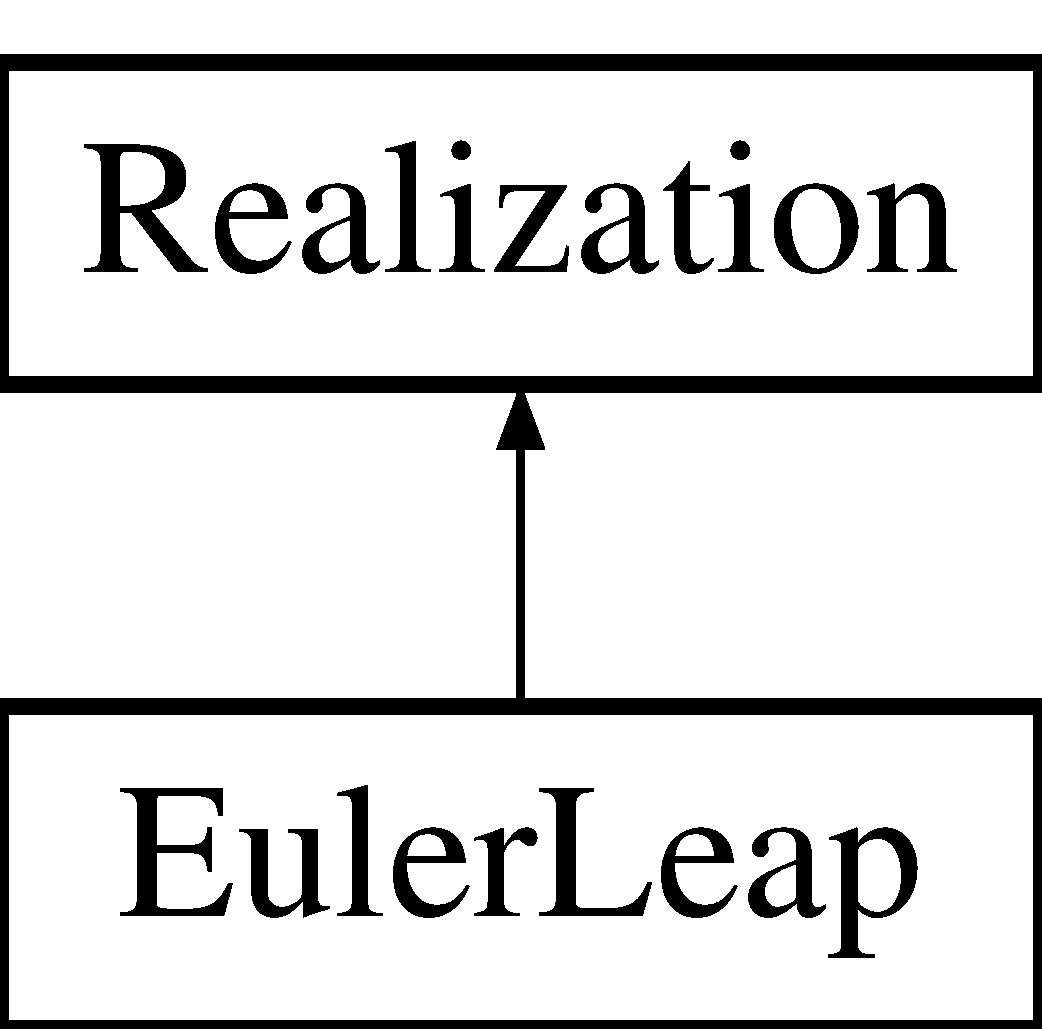
\includegraphics[height=2.000000cm]{class_euler_leap}
\end{center}
\end{figure}
\subsection*{Public Member Functions}
\begin{DoxyCompactItemize}
\item 
\mbox{\Hypertarget{class_euler_leap_ae5db6ea05659798b624a28872799b906}\label{class_euler_leap_ae5db6ea05659798b624a28872799b906}} 
{\bfseries Euler\+Leap} (\hyperlink{class_model}{Model} $\ast$\hyperlink{class_realization_a47ec1d062b8caee874b08c1a17d6aeeb}{the\+\_\+model}, const \hyperlink{class_paramset}{Paramset} \&\hyperlink{class_realization_a119bb29de88929bc51bc1b329473a94b}{the\+\_\+paramset}, \hyperlink{classrng}{rng} $\ast$\hyperlink{class_realization_ac8d358d929afae90cf5790675b6744f9}{the\+\_\+rng}, int \hyperlink{class_realization_ad9951a0829e68e12fcb3817735bb5097}{n\+\_\+vars}, int \hyperlink{class_realization_afb711282bef806fc0020f91252d1df2c}{n\+\_\+events})
\item 
\mbox{\Hypertarget{class_euler_leap_a25b1ea90a95bfd41ecb919605683da9d}\label{class_euler_leap_a25b1ea90a95bfd41ecb919605683da9d}} 
int \hyperlink{class_euler_leap_a25b1ea90a95bfd41ecb919605683da9d}{step} ()
\begin{DoxyCompactList}\small\item\em takes one simulation step according to the chosen algorithm \end{DoxyCompactList}\item 
int \hyperlink{class_euler_leap_a1a13929ea1ebf40e7357439968828f4b}{set\+\_\+to\+\_\+initial\+\_\+state} ()
\begin{DoxyCompactList}\small\item\em Sets state\+\_\+array and state\+\_\+time to their user-\/specified initial values. \end{DoxyCompactList}\end{DoxyCompactItemize}
\subsection*{Additional Inherited Members}


\subsection{Detailed Description}
Class \hyperlink{class_euler_leap}{Euler\+Leap} implements \hyperlink{class_realization}{Realization} \hyperlink{class_euler_leap_a25b1ea90a95bfd41ecb919605683da9d}{step()} function using the basic tau leap approximate algorithm of Gillepsie (2001). The method is analogous to the deterministic forward Euler method the numerical solution of ordinary differential equations. 

\subsection{Member Function Documentation}
\mbox{\Hypertarget{class_euler_leap_a1a13929ea1ebf40e7357439968828f4b}\label{class_euler_leap_a1a13929ea1ebf40e7357439968828f4b}} 
\index{Euler\+Leap@{Euler\+Leap}!set\+\_\+to\+\_\+initial\+\_\+state@{set\+\_\+to\+\_\+initial\+\_\+state}}
\index{set\+\_\+to\+\_\+initial\+\_\+state@{set\+\_\+to\+\_\+initial\+\_\+state}!Euler\+Leap@{Euler\+Leap}}
\subsubsection{\texorpdfstring{set\+\_\+to\+\_\+initial\+\_\+state()}{set\_to\_initial\_state()}}
{\footnotesize\ttfamily int Euler\+Leap\+::set\+\_\+to\+\_\+initial\+\_\+state (\begin{DoxyParamCaption}{ }\end{DoxyParamCaption})\hspace{0.3cm}{\ttfamily [virtual]}}



Sets state\+\_\+array and state\+\_\+time to their user-\/specified initial values. 

\begin{DoxyReturn}{Returns}
int 
\end{DoxyReturn}


Reimplemented from \hyperlink{class_realization_a391a89af7574a9053f53f8a299c2cc70}{Realization}.



The documentation for this class was generated from the following files\+:\begin{DoxyCompactItemize}
\item 
/\+Users/\+Caleb/\+A\+P\+C524/stoched/src/\hyperlink{eulerleap_8h}{eulerleap.\+h}\item 
/\+Users/\+Caleb/\+A\+P\+C524/stoched/src/\hyperlink{eulerleap_8cc}{eulerleap.\+cc}\end{DoxyCompactItemize}

\hypertarget{class_event}{}\section{Event Class Reference}
\label{class_event}\index{Event@{Event}}


Class \hyperlink{class_event}{Event} holds a user-\/specified event, namely set of functions and associated rate.  




{\ttfamily \#include $<$event.\+h$>$}

\subsection*{Public Member Functions}
\begin{DoxyCompactItemize}
\item 
\hyperlink{class_event_a5a40dd4708297f7031e29b39e039ae10}{Event} ()
\begin{DoxyCompactList}\small\item\em Default constructor for \hyperlink{class_event}{Event}. \end{DoxyCompactList}\item 
\hyperlink{class_event_a7704ec01ce91e673885792054214b3d2}{$\sim$\+Event} ()
\begin{DoxyCompactList}\small\item\em Destructor of \hyperlink{class_event}{Event}. \end{DoxyCompactList}\item 
void \hyperlink{class_event_ad380e41418d2e34b651e052711fefe83}{add\+Function} (string function, string variables)
\begin{DoxyCompactList}\small\item\em Add a function parser to the function array. \end{DoxyCompactList}\item 
double \hyperlink{class_event_a2637844b7f9583caf0f808c898dc2246}{use\+Function} (int i\+Function, double $\ast$args)
\begin{DoxyCompactList}\small\item\em Evaluate function stored at specified spot in the function array. \end{DoxyCompactList}\item 
void \hyperlink{class_event_a993a01984496bc158be92b67422f8655}{set\+Rate} (string function, string variables)
\begin{DoxyCompactList}\small\item\em Set equation for rate\+Function. \end{DoxyCompactList}\item 
double \hyperlink{class_event_a2288e3b3fa19e076e04bba11b88d189a}{get\+Rate} (double $\ast$args)
\begin{DoxyCompactList}\small\item\em Return rate to user based on values of the state array. \end{DoxyCompactList}\item 
int \hyperlink{class_event_a1a0f2e2dc0b203f7be0f1d5b8810c6a2}{get\+Size} ()
\begin{DoxyCompactList}\small\item\em Return size of event, namely number of functions, to user. \end{DoxyCompactList}\item 
double \hyperlink{class_event_afb753b1954fd16e7ba92ae16157f70fd}{get\+Delta\+Var} (int i)
\begin{DoxyCompactList}\small\item\em Return how the ith variable is incremented when the ith equation is called. \end{DoxyCompactList}\item 
void \hyperlink{class_event_a980f39895f2afc1c2273d921d92aeac0}{set\+Delta\+Var} (int i, double val)
\begin{DoxyCompactList}\small\item\em set the amount that the ith function increments the ith variable. This is used by midpoint tau leaping \end{DoxyCompactList}\end{DoxyCompactItemize}
\subsection*{Public Attributes}
\begin{DoxyCompactItemize}
\item 
\mbox{\Hypertarget{class_event_acf8fc6215a0eeaa049e2aca9a347f4b0}\label{class_event_acf8fc6215a0eeaa049e2aca9a347f4b0}} 
string {\bfseries event\+Name}
\end{DoxyCompactItemize}
\subsection*{Private Attributes}
\begin{DoxyCompactItemize}
\item 
\mbox{\Hypertarget{class_event_a77f230a68021756fd1e2d35dcfa534f8}\label{class_event_a77f230a68021756fd1e2d35dcfa534f8}} 
Function\+Parser $\ast$$\ast$ \hyperlink{class_event_a77f230a68021756fd1e2d35dcfa534f8}{function\+Array\+\_\+}
\begin{DoxyCompactList}\small\item\em Array of function parsers. \end{DoxyCompactList}\item 
\mbox{\Hypertarget{class_event_a5a82a70465e39626ad62d1cfe3fc7617}\label{class_event_a5a82a70465e39626ad62d1cfe3fc7617}} 
Function\+Parser \hyperlink{class_event_a5a82a70465e39626ad62d1cfe3fc7617}{rate\+Function}
\begin{DoxyCompactList}\small\item\em Rate specified by an equation. \end{DoxyCompactList}\item 
\mbox{\Hypertarget{class_event_a59244ccd0e0f3654f07715bb3dd6423f}\label{class_event_a59244ccd0e0f3654f07715bb3dd6423f}} 
int \hyperlink{class_event_a59244ccd0e0f3654f07715bb3dd6423f}{eq\+\_\+count\+\_\+}
\begin{DoxyCompactList}\small\item\em Number of function parsers. \end{DoxyCompactList}\item 
\mbox{\Hypertarget{class_event_a869e25f5b77f85372eb0397ea01e25bf}\label{class_event_a869e25f5b77f85372eb0397ea01e25bf}} 
double $\ast$ \hyperlink{class_event_a869e25f5b77f85372eb0397ea01e25bf}{delta\+Var\+\_\+}
\begin{DoxyCompactList}\small\item\em how much each variable in the state changes when its corrsponding function is called. Only used by midpoint tau leaping to calculate approximate continuous time derivative. \end{DoxyCompactList}\end{DoxyCompactItemize}


\subsection{Detailed Description}
Class \hyperlink{class_event}{Event} holds a user-\/specified event, namely set of functions and associated rate. 

\subsection{Constructor \& Destructor Documentation}
\mbox{\Hypertarget{class_event_a5a40dd4708297f7031e29b39e039ae10}\label{class_event_a5a40dd4708297f7031e29b39e039ae10}} 
\index{Event@{Event}!Event@{Event}}
\index{Event@{Event}!Event@{Event}}
\subsubsection{\texorpdfstring{Event()}{Event()}}
{\footnotesize\ttfamily Event\+::\+Event (\begin{DoxyParamCaption}{ }\end{DoxyParamCaption})}



Default constructor for \hyperlink{class_event}{Event}. 


\begin{DoxyParams}{Parameters}
{\em eq\+\_\+count} & is the size of the function array \\
\hline
{\em function\+Array} & contains all user-\/specified Function\+Parsers that govern event \\
\hline
\end{DoxyParams}
\begin{DoxyReturn}{Returns}
nothing 
\end{DoxyReturn}
\mbox{\Hypertarget{class_event_a7704ec01ce91e673885792054214b3d2}\label{class_event_a7704ec01ce91e673885792054214b3d2}} 
\index{Event@{Event}!````~Event@{$\sim$\+Event}}
\index{````~Event@{$\sim$\+Event}!Event@{Event}}
\subsubsection{\texorpdfstring{$\sim$\+Event()}{~Event()}}
{\footnotesize\ttfamily Event\+::$\sim$\+Event (\begin{DoxyParamCaption}{ }\end{DoxyParamCaption})}



Destructor of \hyperlink{class_event}{Event}. 

\begin{DoxyReturn}{Returns}
nothing 
\end{DoxyReturn}


\subsection{Member Function Documentation}
\mbox{\Hypertarget{class_event_ad380e41418d2e34b651e052711fefe83}\label{class_event_ad380e41418d2e34b651e052711fefe83}} 
\index{Event@{Event}!add\+Function@{add\+Function}}
\index{add\+Function@{add\+Function}!Event@{Event}}
\subsubsection{\texorpdfstring{add\+Function()}{addFunction()}}
{\footnotesize\ttfamily void Event\+::add\+Function (\begin{DoxyParamCaption}\item[{string}]{function,  }\item[{string}]{variables }\end{DoxyParamCaption})}



Add a function parser to the function array. 


\begin{DoxyParams}{Parameters}
{\em function} & is a string used to generate a Function\+Parser object \\
\hline
{\em variables} & is a string used to generate a Function\+Parser object \\
\hline
\end{DoxyParams}
\begin{DoxyReturn}{Returns}
void 
\end{DoxyReturn}
\mbox{\Hypertarget{class_event_afb753b1954fd16e7ba92ae16157f70fd}\label{class_event_afb753b1954fd16e7ba92ae16157f70fd}} 
\index{Event@{Event}!get\+Delta\+Var@{get\+Delta\+Var}}
\index{get\+Delta\+Var@{get\+Delta\+Var}!Event@{Event}}
\subsubsection{\texorpdfstring{get\+Delta\+Var()}{getDeltaVar()}}
{\footnotesize\ttfamily double Event\+::get\+Delta\+Var (\begin{DoxyParamCaption}\item[{int}]{i }\end{DoxyParamCaption})}



Return how the ith variable is incremented when the ith equation is called. 


\begin{DoxyParams}{Parameters}
{\em i} & is an int specifying of which variable to find the delta. 0 is the first variable \\
\hline
\end{DoxyParams}
\begin{DoxyReturn}{Returns}
change in value of i when its corresponding equation is called, as a double 
\end{DoxyReturn}
\mbox{\Hypertarget{class_event_a2288e3b3fa19e076e04bba11b88d189a}\label{class_event_a2288e3b3fa19e076e04bba11b88d189a}} 
\index{Event@{Event}!get\+Rate@{get\+Rate}}
\index{get\+Rate@{get\+Rate}!Event@{Event}}
\subsubsection{\texorpdfstring{get\+Rate()}{getRate()}}
{\footnotesize\ttfamily double Event\+::get\+Rate (\begin{DoxyParamCaption}\item[{double $\ast$}]{state\+Array }\end{DoxyParamCaption})}



Return rate to user based on values of the state array. 


\begin{DoxyParams}{Parameters}
{\em state\+Array} & is a double array specifying variable values of function \\
\hline
\end{DoxyParams}
\begin{DoxyReturn}{Returns}
evaluated rate\+Function as a double 
\end{DoxyReturn}
\mbox{\Hypertarget{class_event_a1a0f2e2dc0b203f7be0f1d5b8810c6a2}\label{class_event_a1a0f2e2dc0b203f7be0f1d5b8810c6a2}} 
\index{Event@{Event}!get\+Size@{get\+Size}}
\index{get\+Size@{get\+Size}!Event@{Event}}
\subsubsection{\texorpdfstring{get\+Size()}{getSize()}}
{\footnotesize\ttfamily int Event\+::get\+Size (\begin{DoxyParamCaption}{ }\end{DoxyParamCaption})}



Return size of event, namely number of functions, to user. 

\begin{DoxyReturn}{Returns}
size of event, namely number of functions, as an int 
\end{DoxyReturn}
\mbox{\Hypertarget{class_event_a980f39895f2afc1c2273d921d92aeac0}\label{class_event_a980f39895f2afc1c2273d921d92aeac0}} 
\index{Event@{Event}!set\+Delta\+Var@{set\+Delta\+Var}}
\index{set\+Delta\+Var@{set\+Delta\+Var}!Event@{Event}}
\subsubsection{\texorpdfstring{set\+Delta\+Var()}{setDeltaVar()}}
{\footnotesize\ttfamily void Event\+::set\+Delta\+Var (\begin{DoxyParamCaption}\item[{int}]{i,  }\item[{double}]{val }\end{DoxyParamCaption})}



set the amount that the ith function increments the ith variable. This is used by midpoint tau leaping 


\begin{DoxyParams}{Parameters}
{\em i} & is an int specifying of which variable to set. 0 is the first variable \\
\hline
\end{DoxyParams}
\begin{DoxyReturn}{Returns}
void 
\end{DoxyReturn}
\mbox{\Hypertarget{class_event_a993a01984496bc158be92b67422f8655}\label{class_event_a993a01984496bc158be92b67422f8655}} 
\index{Event@{Event}!set\+Rate@{set\+Rate}}
\index{set\+Rate@{set\+Rate}!Event@{Event}}
\subsubsection{\texorpdfstring{set\+Rate()}{setRate()}}
{\footnotesize\ttfamily void Event\+::set\+Rate (\begin{DoxyParamCaption}\item[{string}]{function,  }\item[{string}]{variables }\end{DoxyParamCaption})}



Set equation for rate\+Function. 


\begin{DoxyParams}{Parameters}
{\em function} & is a string used for parsing rate\+Function \\
\hline
{\em variables} & is a string used for parsing rate\+Function \\
\hline
\end{DoxyParams}
\begin{DoxyReturn}{Returns}
void 
\end{DoxyReturn}
\mbox{\Hypertarget{class_event_a2637844b7f9583caf0f808c898dc2246}\label{class_event_a2637844b7f9583caf0f808c898dc2246}} 
\index{Event@{Event}!use\+Function@{use\+Function}}
\index{use\+Function@{use\+Function}!Event@{Event}}
\subsubsection{\texorpdfstring{use\+Function()}{useFunction()}}
{\footnotesize\ttfamily double Event\+::use\+Function (\begin{DoxyParamCaption}\item[{int}]{i\+Function,  }\item[{double $\ast$}]{state\+Array }\end{DoxyParamCaption})}



Evaluate function stored at specified spot in the function array. 


\begin{DoxyParams}{Parameters}
{\em i\+Function} & is an int that indexes function array \\
\hline
{\em state\+Array} & is a double array specifying variable values of function \\
\hline
\end{DoxyParams}
\begin{DoxyReturn}{Returns}
evaluated function\+Parser as a double 
\end{DoxyReturn}


The documentation for this class was generated from the following files\+:\begin{DoxyCompactItemize}
\item 
/\+Users/dylan/stoched/src/\hyperlink{event_8h}{event.\+h}\item 
/\+Users/dylan/stoched/src/\hyperlink{event_8cc}{event.\+cc}\end{DoxyCompactItemize}

\hypertarget{class_first_reaction}{}\section{First\+Reaction Class Reference}
\label{class_first_reaction}\index{First\+Reaction@{First\+Reaction}}
Inheritance diagram for First\+Reaction\+:\begin{figure}[H]
\begin{center}
\leavevmode
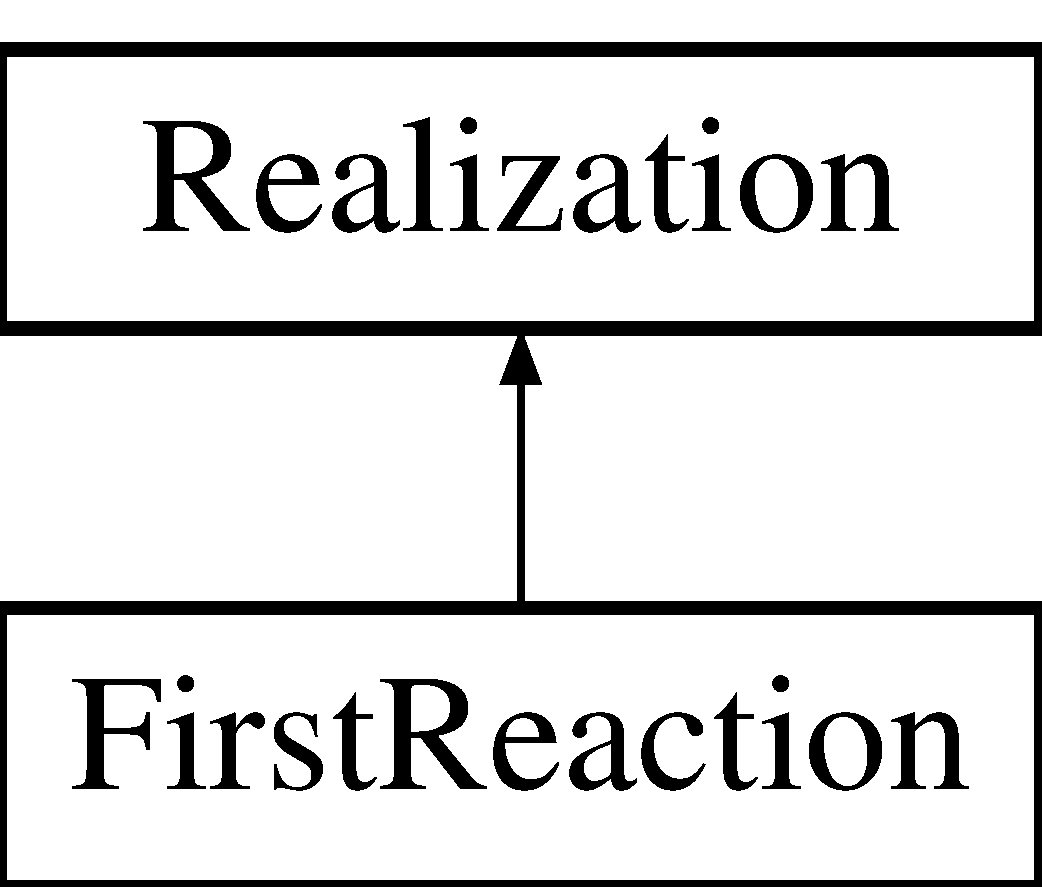
\includegraphics[height=2.000000cm]{class_first_reaction}
\end{center}
\end{figure}
\subsection*{Public Member Functions}
\begin{DoxyCompactItemize}
\item 
\mbox{\Hypertarget{class_first_reaction_a5122d48f6ecbe17a75cecd41b06ac4a2}\label{class_first_reaction_a5122d48f6ecbe17a75cecd41b06ac4a2}} 
{\bfseries First\+Reaction} (\hyperlink{class_model}{Model} $\ast$\hyperlink{class_realization_a47ec1d062b8caee874b08c1a17d6aeeb}{the\+\_\+model}, const \hyperlink{class_paramset}{Paramset} \&\hyperlink{class_realization_a119bb29de88929bc51bc1b329473a94b}{the\+\_\+paramset}, \hyperlink{classrng}{rng} $\ast$the\+\_\+rng, int n\+\_\+vars, int n\+\_\+events)
\item 
\mbox{\Hypertarget{class_first_reaction_aed63c3c95d20b2ad557dabb6c5376a73}\label{class_first_reaction_aed63c3c95d20b2ad557dabb6c5376a73}} 
int \hyperlink{class_first_reaction_aed63c3c95d20b2ad557dabb6c5376a73}{step} ()
\begin{DoxyCompactList}\small\item\em takes one simulation step according to the chosen algorithm \end{DoxyCompactList}\end{DoxyCompactItemize}
\subsection*{Private Attributes}
\begin{DoxyCompactItemize}
\item 
\mbox{\Hypertarget{class_first_reaction_adef190a1cb589cc8317b469f94cd6ad4}\label{class_first_reaction_adef190a1cb589cc8317b469f94cd6ad4}} 
double $\ast$ {\bfseries waiting\+\_\+times}
\end{DoxyCompactItemize}
\subsection*{Additional Inherited Members}


The documentation for this class was generated from the following files\+:\begin{DoxyCompactItemize}
\item 
/\+Users/\+Caleb/\+A\+P\+C524/stoched/src/\hyperlink{realization_8h}{realization.\+h}\item 
/\+Users/\+Caleb/\+A\+P\+C524/stoched/src/\hyperlink{realization_8cc}{realization.\+cc}\end{DoxyCompactItemize}

\hypertarget{class_midpoint_leap}{}\section{Midpoint\+Leap Class Reference}
\label{class_midpoint_leap}\index{Midpoint\+Leap@{Midpoint\+Leap}}


Class \hyperlink{class_midpoint_leap}{Midpoint\+Leap} implements \hyperlink{class_realization}{Realization} \hyperlink{class_midpoint_leap_a8afc1a6a8777157f7b42ec08a848b564}{step()} function using the midpoint tau leap approximate algorithm of Gillepsie (2001). The method is analogous to the deterministic midpoint (2nd-\/order Runge-\/\+Kutta) method for the numerical solution of ordinary differential equations.  




{\ttfamily \#include $<$midpointleap.\+h$>$}

Inheritance diagram for Midpoint\+Leap\+:\begin{figure}[H]
\begin{center}
\leavevmode
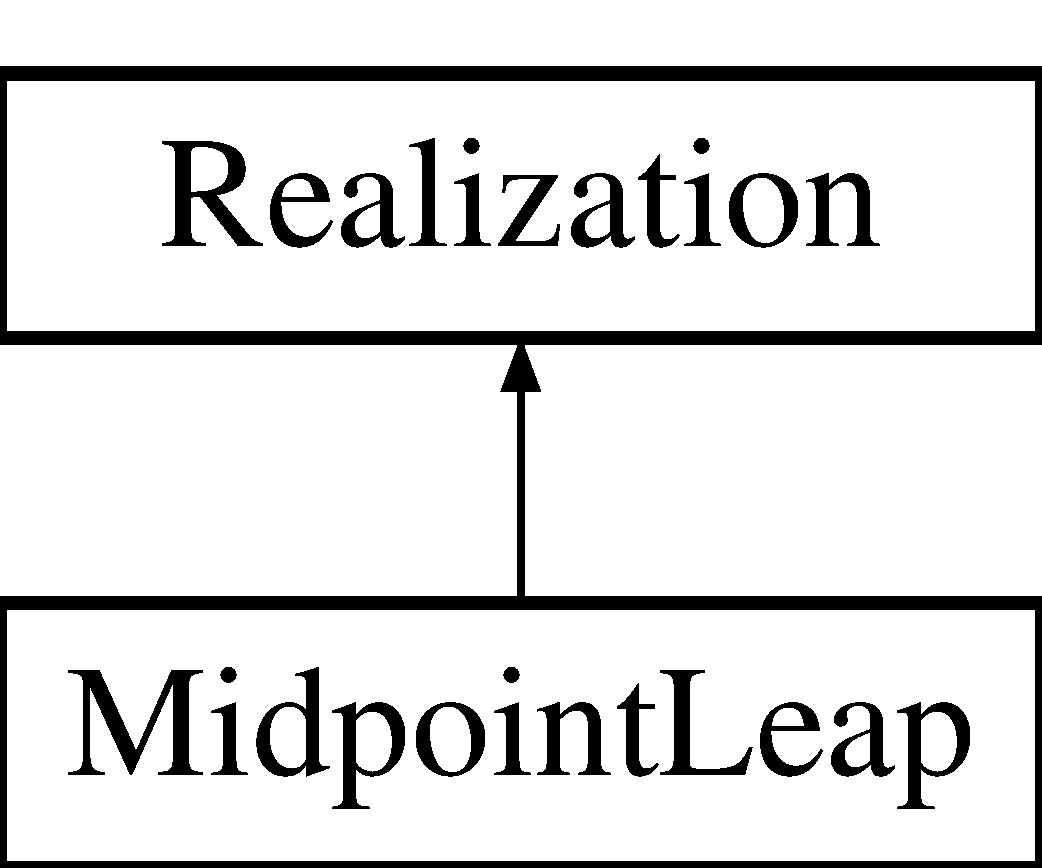
\includegraphics[height=2.000000cm]{class_midpoint_leap}
\end{center}
\end{figure}
\subsection*{Public Member Functions}
\begin{DoxyCompactItemize}
\item 
\hyperlink{class_midpoint_leap_a9e5301b74a349ecc4c1de994426eb8b2}{Midpoint\+Leap} (\hyperlink{class_model}{Model} $\ast$\hyperlink{class_realization_a47ec1d062b8caee874b08c1a17d6aeeb}{the\+\_\+model}, const \hyperlink{class_paramset}{Paramset} \&\hyperlink{class_realization_a119bb29de88929bc51bc1b329473a94b}{the\+\_\+paramset}, \hyperlink{classrng}{rng} $\ast$\hyperlink{class_realization_ac8d358d929afae90cf5790675b6744f9}{the\+\_\+rng}, int \hyperlink{class_realization_ad9951a0829e68e12fcb3817735bb5097}{n\+\_\+vars}, int \hyperlink{class_realization_afb711282bef806fc0020f91252d1df2c}{n\+\_\+events})
\begin{DoxyCompactList}\small\item\em Default constructor for \hyperlink{class_midpoint_leap}{Midpoint\+Leap}. \end{DoxyCompactList}\item 
\hyperlink{class_midpoint_leap_ae220cffbf343b380ef53e8a2749327f6}{$\sim$\+Midpoint\+Leap} ()
\begin{DoxyCompactList}\small\item\em Destructor for \hyperlink{class_midpoint_leap}{Midpoint\+Leap}. \end{DoxyCompactList}\item 
int \hyperlink{class_midpoint_leap_a8afc1a6a8777157f7b42ec08a848b564}{step} ()
\begin{DoxyCompactList}\small\item\em Update waiting times. \end{DoxyCompactList}\item 
int \hyperlink{class_midpoint_leap_a177682cf5042407ccee1a443e8920896}{set\+\_\+to\+\_\+initial\+\_\+state} ()
\begin{DoxyCompactList}\small\item\em Sets state\+\_\+array and state\+\_\+time to their user-\/specified initial values. \end{DoxyCompactList}\end{DoxyCompactItemize}
\subsection*{Private Attributes}
\begin{DoxyCompactItemize}
\item 
\mbox{\Hypertarget{class_midpoint_leap_abf06466b009f0e52938cbf8fd299f406}\label{class_midpoint_leap_abf06466b009f0e52938cbf8fd299f406}} 
double $\ast$ \hyperlink{class_midpoint_leap_abf06466b009f0e52938cbf8fd299f406}{midpoint\+\_\+array\+\_\+}
\begin{DoxyCompactList}\small\item\em midpoint\+\_\+array\+\_\+ is a double array holding the current midpoints for the tau-\/leap step \end{DoxyCompactList}\end{DoxyCompactItemize}
\subsection*{Additional Inherited Members}


\subsection{Detailed Description}
Class \hyperlink{class_midpoint_leap}{Midpoint\+Leap} implements \hyperlink{class_realization}{Realization} \hyperlink{class_midpoint_leap_a8afc1a6a8777157f7b42ec08a848b564}{step()} function using the midpoint tau leap approximate algorithm of Gillepsie (2001). The method is analogous to the deterministic midpoint (2nd-\/order Runge-\/\+Kutta) method for the numerical solution of ordinary differential equations. 

\subsection{Constructor \& Destructor Documentation}
\mbox{\Hypertarget{class_midpoint_leap_a9e5301b74a349ecc4c1de994426eb8b2}\label{class_midpoint_leap_a9e5301b74a349ecc4c1de994426eb8b2}} 
\index{Midpoint\+Leap@{Midpoint\+Leap}!Midpoint\+Leap@{Midpoint\+Leap}}
\index{Midpoint\+Leap@{Midpoint\+Leap}!Midpoint\+Leap@{Midpoint\+Leap}}
\subsubsection{\texorpdfstring{Midpoint\+Leap()}{MidpointLeap()}}
{\footnotesize\ttfamily Midpoint\+Leap\+::\+Midpoint\+Leap (\begin{DoxyParamCaption}\item[{\hyperlink{class_model}{Model} $\ast$}]{the\+\_\+model,  }\item[{const \hyperlink{class_paramset}{Paramset} \&}]{the\+\_\+paramset,  }\item[{\hyperlink{classrng}{rng} $\ast$}]{the\+\_\+rng,  }\item[{int}]{n\+\_\+vars,  }\item[{int}]{n\+\_\+events }\end{DoxyParamCaption})}



Default constructor for \hyperlink{class_midpoint_leap}{Midpoint\+Leap}. 


\begin{DoxyParams}{Parameters}
{\em the\+\_\+model} & is a \hyperlink{class_model}{Model} object \\
\hline
{\em the\+\_\+paramset} & is a \hyperlink{class_paramset}{Paramset} object \\
\hline
{\em the\+\_\+rng} & is a random number generator \\
\hline
{\em n\+\_\+vars} & is an int specifying variable count \\
\hline
{\em n\+\_\+events} & is an int specifying event count\\
\hline
\end{DoxyParams}
\begin{DoxyReturn}{Returns}
nothing 
\end{DoxyReturn}
intialize midpoint array \mbox{\Hypertarget{class_midpoint_leap_ae220cffbf343b380ef53e8a2749327f6}\label{class_midpoint_leap_ae220cffbf343b380ef53e8a2749327f6}} 
\index{Midpoint\+Leap@{Midpoint\+Leap}!````~Midpoint\+Leap@{$\sim$\+Midpoint\+Leap}}
\index{````~Midpoint\+Leap@{$\sim$\+Midpoint\+Leap}!Midpoint\+Leap@{Midpoint\+Leap}}
\subsubsection{\texorpdfstring{$\sim$\+Midpoint\+Leap()}{~MidpointLeap()}}
{\footnotesize\ttfamily Midpoint\+Leap\+::$\sim$\+Midpoint\+Leap (\begin{DoxyParamCaption}{ }\end{DoxyParamCaption})}



Destructor for \hyperlink{class_midpoint_leap}{Midpoint\+Leap}. 

\begin{DoxyReturn}{Returns}
nothing 
\end{DoxyReturn}


\subsection{Member Function Documentation}
\mbox{\Hypertarget{class_midpoint_leap_a177682cf5042407ccee1a443e8920896}\label{class_midpoint_leap_a177682cf5042407ccee1a443e8920896}} 
\index{Midpoint\+Leap@{Midpoint\+Leap}!set\+\_\+to\+\_\+initial\+\_\+state@{set\+\_\+to\+\_\+initial\+\_\+state}}
\index{set\+\_\+to\+\_\+initial\+\_\+state@{set\+\_\+to\+\_\+initial\+\_\+state}!Midpoint\+Leap@{Midpoint\+Leap}}
\subsubsection{\texorpdfstring{set\+\_\+to\+\_\+initial\+\_\+state()}{set\_to\_initial\_state()}}
{\footnotesize\ttfamily int Midpoint\+Leap\+::set\+\_\+to\+\_\+initial\+\_\+state (\begin{DoxyParamCaption}{ }\end{DoxyParamCaption})\hspace{0.3cm}{\ttfamily [virtual]}}



Sets state\+\_\+array and state\+\_\+time to their user-\/specified initial values. 

\begin{DoxyReturn}{Returns}
int 
\end{DoxyReturn}


Reimplemented from \hyperlink{class_realization_a391a89af7574a9053f53f8a299c2cc70}{Realization}.

\mbox{\Hypertarget{class_midpoint_leap_a8afc1a6a8777157f7b42ec08a848b564}\label{class_midpoint_leap_a8afc1a6a8777157f7b42ec08a848b564}} 
\index{Midpoint\+Leap@{Midpoint\+Leap}!step@{step}}
\index{step@{step}!Midpoint\+Leap@{Midpoint\+Leap}}
\subsubsection{\texorpdfstring{step()}{step()}}
{\footnotesize\ttfamily int Midpoint\+Leap\+::step (\begin{DoxyParamCaption}{ }\end{DoxyParamCaption})\hspace{0.3cm}{\ttfamily [virtual]}}



Update waiting times. 

\begin{DoxyReturn}{Returns}
int 
\end{DoxyReturn}


Implements \hyperlink{class_realization_a9949217117927b149850288f3b74c9ef}{Realization}.



The documentation for this class was generated from the following files\+:\begin{DoxyCompactItemize}
\item 
/\+Users/\+Caleb/\+A\+P\+C524/stoched/src/\hyperlink{midpointleap_8h}{midpointleap.\+h}\item 
/\+Users/\+Caleb/\+A\+P\+C524/stoched/src/\hyperlink{midpointleap_8cc}{midpointleap.\+cc}\end{DoxyCompactItemize}

\hypertarget{class_model}{}\section{Model Class Reference}
\label{class_model}\index{Model@{Model}}


Class M\+O\+D\+EL, which holds user-\/specified models of stochastic systems from which realizations are to be simulated. A model may have variable parameters; each complete set will be stored in an object of class \hyperlink{class_paramset}{Paramset}.  




{\ttfamily \#include $<$model.\+h$>$}

\subsection*{Public Member Functions}
\begin{DoxyCompactItemize}
\item 
\hyperlink{class_model_ae3b375de5f6df4faf74a95d64748e048}{Model} ()
\begin{DoxyCompactList}\small\item\em Default constructor for \hyperlink{class_model}{Model}. \end{DoxyCompactList}\item 
\hyperlink{class_model_ad6ebd2062a0b823db841a0b88baac4c0}{$\sim$\+Model} ()
\begin{DoxyCompactList}\small\item\em Destructor of \hyperlink{class_model}{Model}. \end{DoxyCompactList}\item 
void \hyperlink{class_model_a4743b4f267eeb1a60e21cc2995e1efcd}{add\+Vars} (string vars)
\begin{DoxyCompactList}\small\item\em Add variable list to a \hyperlink{class_model}{Model}. \end{DoxyCompactList}\item 
void \hyperlink{class_model_ab6f784e4ff8cdf3ee5e010ef4dd8d597}{add\+Event} (string function\+Rate)
\begin{DoxyCompactList}\small\item\em Add \hyperlink{class_event}{Event} to \hyperlink{class_model}{Model}\textquotesingle{}s list of Events. \end{DoxyCompactList}\item 
void \hyperlink{class_model_a78d9b07bd5e819215c9aeefabb4cede7}{add\+Event\+Fct} (int i\+Event, string function)
\begin{DoxyCompactList}\small\item\em Add \hyperlink{class_event}{Event} function to specified \hyperlink{class_event}{Event} in \hyperlink{class_model}{Model}. \end{DoxyCompactList}\item 
double \hyperlink{class_model_a774d9fb034f8704a75d7b3568a87a3bc}{use\+Event\+Fct} (int i\+Event, int i\+Function, double $\ast$state\+Array)
\begin{DoxyCompactList}\small\item\em Evaluate given function in specified \hyperlink{class_event}{Event}. \end{DoxyCompactList}\item 
double \hyperlink{class_model_a2909caddddccca90faaae708e68226ad}{get\+Event\+Rate} (int i\+Event, double $\ast$state\+Array)
\begin{DoxyCompactList}\small\item\em Evaluate rate function for a specified \hyperlink{class_event}{Event}. \end{DoxyCompactList}\item 
void \hyperlink{class_model_ad9e7a181a31a2a9fab052d11b1984afd}{update\+State} (int i\+Event, double $\ast$state\+Array)
\begin{DoxyCompactList}\small\item\em Update state array by evaluating all functions of a given \hyperlink{class_event}{Event}. \end{DoxyCompactList}\item 
void \hyperlink{class_model_a3f2fd71261c87162718864d7efc67f2f}{update\+Rates} (double $\ast$state\+Array, double $\ast$rate\+Array)
\begin{DoxyCompactList}\small\item\em Update rate for all Events in \hyperlink{class_model}{Model}\textquotesingle{}s \hyperlink{class_event}{Event} list. \end{DoxyCompactList}\end{DoxyCompactItemize}


\subsection{Detailed Description}
Class M\+O\+D\+EL, which holds user-\/specified models of stochastic systems from which realizations are to be simulated. A model may have variable parameters; each complete set will be stored in an object of class \hyperlink{class_paramset}{Paramset}. 

\subsection{Constructor \& Destructor Documentation}
\mbox{\Hypertarget{class_model_ae3b375de5f6df4faf74a95d64748e048}\label{class_model_ae3b375de5f6df4faf74a95d64748e048}} 
\index{Model@{Model}!Model@{Model}}
\index{Model@{Model}!Model@{Model}}
\subsubsection{\texorpdfstring{Model()}{Model()}}
{\footnotesize\ttfamily Model\+::\+Model (\begin{DoxyParamCaption}{ }\end{DoxyParamCaption})}



Default constructor for \hyperlink{class_model}{Model}. 


\begin{DoxyParams}{Parameters}
{\em none} & \\
\hline
\end{DoxyParams}
\begin{DoxyReturn}{Returns}
nothing 
\end{DoxyReturn}
\mbox{\Hypertarget{class_model_ad6ebd2062a0b823db841a0b88baac4c0}\label{class_model_ad6ebd2062a0b823db841a0b88baac4c0}} 
\index{Model@{Model}!````~Model@{$\sim$\+Model}}
\index{````~Model@{$\sim$\+Model}!Model@{Model}}
\subsubsection{\texorpdfstring{$\sim$\+Model()}{~Model()}}
{\footnotesize\ttfamily Model\+::$\sim$\+Model (\begin{DoxyParamCaption}{ }\end{DoxyParamCaption})}



Destructor of \hyperlink{class_model}{Model}. 


\begin{DoxyParams}{Parameters}
{\em none} & \\
\hline
\end{DoxyParams}
\begin{DoxyReturn}{Returns}
nothing 
\end{DoxyReturn}


\subsection{Member Function Documentation}
\mbox{\Hypertarget{class_model_ab6f784e4ff8cdf3ee5e010ef4dd8d597}\label{class_model_ab6f784e4ff8cdf3ee5e010ef4dd8d597}} 
\index{Model@{Model}!add\+Event@{add\+Event}}
\index{add\+Event@{add\+Event}!Model@{Model}}
\subsubsection{\texorpdfstring{add\+Event()}{addEvent()}}
{\footnotesize\ttfamily void Model\+::add\+Event (\begin{DoxyParamCaption}\item[{string}]{function\+Rate }\end{DoxyParamCaption})}



Add \hyperlink{class_event}{Event} to \hyperlink{class_model}{Model}\textquotesingle{}s list of Events. 


\begin{DoxyParams}{Parameters}
{\em function\+Rate} & is a string that defines an \hyperlink{class_event}{Event}\textquotesingle{}s rate \\
\hline
\end{DoxyParams}
\begin{DoxyReturn}{Returns}
void 
\end{DoxyReturn}
\mbox{\Hypertarget{class_model_a78d9b07bd5e819215c9aeefabb4cede7}\label{class_model_a78d9b07bd5e819215c9aeefabb4cede7}} 
\index{Model@{Model}!add\+Event\+Fct@{add\+Event\+Fct}}
\index{add\+Event\+Fct@{add\+Event\+Fct}!Model@{Model}}
\subsubsection{\texorpdfstring{add\+Event\+Fct()}{addEventFct()}}
{\footnotesize\ttfamily void Model\+::add\+Event\+Fct (\begin{DoxyParamCaption}\item[{int}]{i\+Event,  }\item[{string}]{function }\end{DoxyParamCaption})}



Add \hyperlink{class_event}{Event} function to specified \hyperlink{class_event}{Event} in \hyperlink{class_model}{Model}. 


\begin{DoxyParams}{Parameters}
{\em i\+Event} & is an int that indexes \hyperlink{class_event}{Event} list \\
\hline
{\em function} & is a string that specifies \hyperlink{class_event}{Event} function \\
\hline
\end{DoxyParams}
\begin{DoxyReturn}{Returns}
void 
\end{DoxyReturn}
\mbox{\Hypertarget{class_model_a4743b4f267eeb1a60e21cc2995e1efcd}\label{class_model_a4743b4f267eeb1a60e21cc2995e1efcd}} 
\index{Model@{Model}!add\+Vars@{add\+Vars}}
\index{add\+Vars@{add\+Vars}!Model@{Model}}
\subsubsection{\texorpdfstring{add\+Vars()}{addVars()}}
{\footnotesize\ttfamily void Model\+::add\+Vars (\begin{DoxyParamCaption}\item[{string}]{vars }\end{DoxyParamCaption})}



Add variable list to a \hyperlink{class_model}{Model}. 


\begin{DoxyParams}{Parameters}
{\em vars} & is a string used to set variables associate with a \hyperlink{class_model}{Model} \\
\hline
\end{DoxyParams}
\begin{DoxyReturn}{Returns}
void 
\end{DoxyReturn}
\mbox{\Hypertarget{class_model_a2909caddddccca90faaae708e68226ad}\label{class_model_a2909caddddccca90faaae708e68226ad}} 
\index{Model@{Model}!get\+Event\+Rate@{get\+Event\+Rate}}
\index{get\+Event\+Rate@{get\+Event\+Rate}!Model@{Model}}
\subsubsection{\texorpdfstring{get\+Event\+Rate()}{getEventRate()}}
{\footnotesize\ttfamily double Model\+::get\+Event\+Rate (\begin{DoxyParamCaption}\item[{int}]{i\+Event,  }\item[{double $\ast$}]{state\+Array }\end{DoxyParamCaption})}



Evaluate rate function for a specified \hyperlink{class_event}{Event}. 


\begin{DoxyParams}{Parameters}
{\em i\+Event} & is an int that indexes \hyperlink{class_event}{Event} list \\
\hline
{\em state\+Array} & is a double array specifiying variable values of a function \\
\hline
\end{DoxyParams}
\begin{DoxyReturn}{Returns}
evaluated rate function as a double 
\end{DoxyReturn}
\mbox{\Hypertarget{class_model_a3f2fd71261c87162718864d7efc67f2f}\label{class_model_a3f2fd71261c87162718864d7efc67f2f}} 
\index{Model@{Model}!update\+Rates@{update\+Rates}}
\index{update\+Rates@{update\+Rates}!Model@{Model}}
\subsubsection{\texorpdfstring{update\+Rates()}{updateRates()}}
{\footnotesize\ttfamily void Model\+::update\+Rates (\begin{DoxyParamCaption}\item[{double $\ast$}]{state\+Array,  }\item[{double $\ast$}]{rate\+Array }\end{DoxyParamCaption})}



Update rate for all Events in \hyperlink{class_model}{Model}\textquotesingle{}s \hyperlink{class_event}{Event} list. 


\begin{DoxyParams}{Parameters}
{\em state\+Array} & is a double array specifiying variable values of a function \\
\hline
{\em rate\+Array} & is a double array specifiying variable values of a rate function \\
\hline
\end{DoxyParams}
\begin{DoxyReturn}{Returns}
void 
\end{DoxyReturn}
\mbox{\Hypertarget{class_model_ad9e7a181a31a2a9fab052d11b1984afd}\label{class_model_ad9e7a181a31a2a9fab052d11b1984afd}} 
\index{Model@{Model}!update\+State@{update\+State}}
\index{update\+State@{update\+State}!Model@{Model}}
\subsubsection{\texorpdfstring{update\+State()}{updateState()}}
{\footnotesize\ttfamily void Model\+::update\+State (\begin{DoxyParamCaption}\item[{int}]{i\+Event,  }\item[{double $\ast$}]{state\+Array }\end{DoxyParamCaption})}



Update state array by evaluating all functions of a given \hyperlink{class_event}{Event}. 


\begin{DoxyParams}{Parameters}
{\em i\+Event} & is an int that indexes \hyperlink{class_event}{Event} list \\
\hline
{\em state\+Array} & is a double array specifiying variable values of a function \\
\hline
\end{DoxyParams}
\begin{DoxyReturn}{Returns}
void 
\end{DoxyReturn}
\mbox{\Hypertarget{class_model_a774d9fb034f8704a75d7b3568a87a3bc}\label{class_model_a774d9fb034f8704a75d7b3568a87a3bc}} 
\index{Model@{Model}!use\+Event\+Fct@{use\+Event\+Fct}}
\index{use\+Event\+Fct@{use\+Event\+Fct}!Model@{Model}}
\subsubsection{\texorpdfstring{use\+Event\+Fct()}{useEventFct()}}
{\footnotesize\ttfamily double Model\+::use\+Event\+Fct (\begin{DoxyParamCaption}\item[{int}]{i\+Event,  }\item[{int}]{i\+Function,  }\item[{double $\ast$}]{state\+Array }\end{DoxyParamCaption})}



Evaluate given function in specified \hyperlink{class_event}{Event}. 


\begin{DoxyParams}{Parameters}
{\em i\+Event} & is an int that indexes \hyperlink{class_event}{Event} list \\
\hline
{\em i\+Function} & is an int that indexes an \hyperlink{class_event}{Event}\textquotesingle{}s Function list \\
\hline
{\em state\+Array} & is a double array specifiying variable values of a function \\
\hline
\end{DoxyParams}
\begin{DoxyReturn}{Returns}
evaluated function as a double 
\end{DoxyReturn}


The documentation for this class was generated from the following files\+:\begin{DoxyCompactItemize}
\item 
/\+Users/\+Caleb/\+A\+P\+C524/stoched/src/model.\+h\item 
/\+Users/\+Caleb/\+A\+P\+C524/stoched/src/\hyperlink{model_8cc}{model.\+cc}\end{DoxyCompactItemize}

\hypertarget{class_next_reaction}{}\section{Next\+Reaction Class Reference}
\label{class_next_reaction}\index{Next\+Reaction@{Next\+Reaction}}


Class \hyperlink{class_next_reaction}{Next\+Reaction} implements \hyperlink{class_realization}{Realization} \hyperlink{class_next_reaction_a2c1502879c76efe398c2947056936725}{step()} function using the exact Next Reaction algorithm of Gibson \& Bruck (2000)  




{\ttfamily \#include $<$nextreaction.\+h$>$}

Inheritance diagram for Next\+Reaction\+:\begin{figure}[H]
\begin{center}
\leavevmode
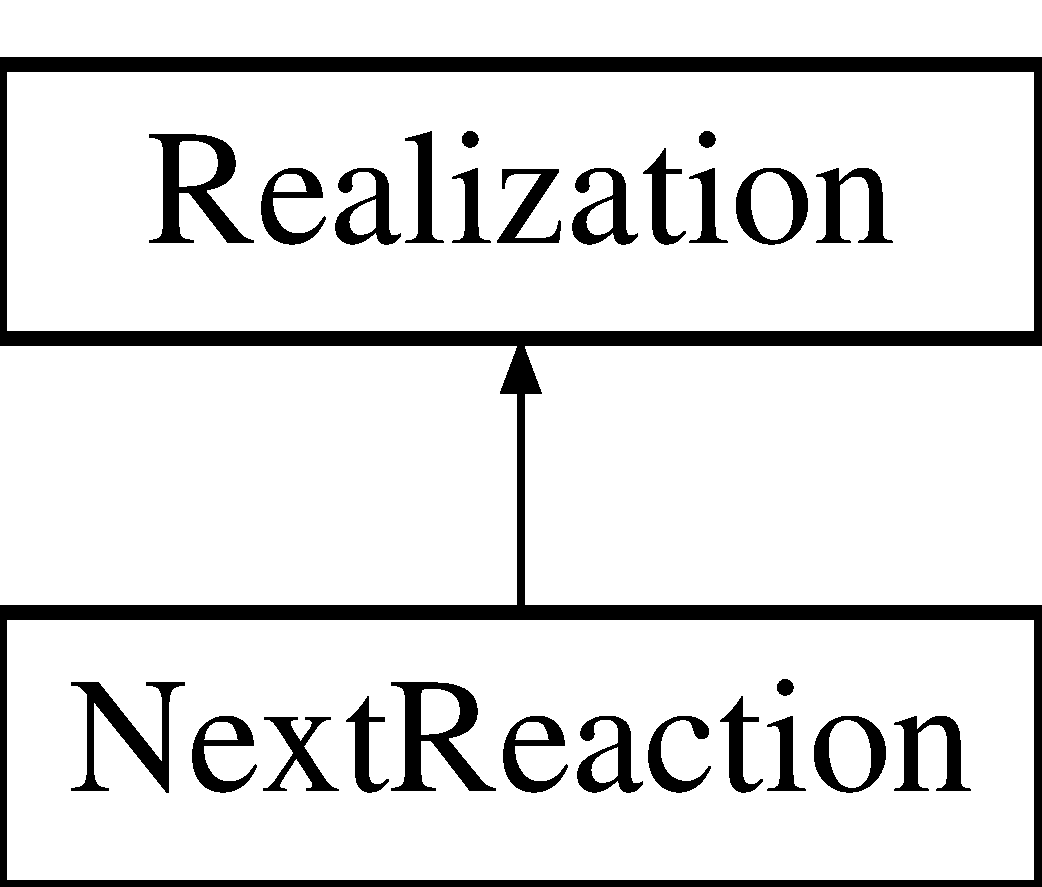
\includegraphics[height=2.000000cm]{class_next_reaction}
\end{center}
\end{figure}
\subsection*{Public Member Functions}
\begin{DoxyCompactItemize}
\item 
\hyperlink{class_next_reaction_ac08695146983c863c3edf3bb4e61d9f9}{Next\+Reaction} (\hyperlink{class_model}{Model} $\ast$\hyperlink{class_realization_a47ec1d062b8caee874b08c1a17d6aeeb}{the\+\_\+model}, const \hyperlink{class_paramset}{Paramset} \&\hyperlink{class_realization_a119bb29de88929bc51bc1b329473a94b}{the\+\_\+paramset}, \hyperlink{classrng}{rng} $\ast$\hyperlink{class_realization_ac8d358d929afae90cf5790675b6744f9}{the\+\_\+rng}, int \hyperlink{class_realization_ad9951a0829e68e12fcb3817735bb5097}{n\+\_\+vars}, int \hyperlink{class_realization_afb711282bef806fc0020f91252d1df2c}{n\+\_\+events})
\begin{DoxyCompactList}\small\item\em Default constructor for \hyperlink{class_next_reaction}{Next\+Reaction}. \end{DoxyCompactList}\item 
\hyperlink{class_next_reaction_aceb23c3b2e23c811809ef04197a39e8d}{$\sim$\+Next\+Reaction} ()
\begin{DoxyCompactList}\small\item\em Destructor for \hyperlink{class_next_reaction}{Next\+Reaction}. \end{DoxyCompactList}\item 
int \hyperlink{class_next_reaction_a2c1502879c76efe398c2947056936725}{step} ()
\begin{DoxyCompactList}\small\item\em Update waiting times. \end{DoxyCompactList}\item 
int \hyperlink{class_next_reaction_a0cc63c4ec9fe3f338472fff302f6d746}{set\+\_\+to\+\_\+initial\+\_\+state} ()
\begin{DoxyCompactList}\small\item\em Sets state\+\_\+array and state\+\_\+time to their user-\/specified initial values. \end{DoxyCompactList}\end{DoxyCompactItemize}
\subsection*{Private Attributes}
\begin{DoxyCompactItemize}
\item 
\mbox{\Hypertarget{class_next_reaction_a8a7d82a004db70828dd732bf57cf35b6}\label{class_next_reaction_a8a7d82a004db70828dd732bf57cf35b6}} 
double $\ast$ \hyperlink{class_next_reaction_a8a7d82a004db70828dd732bf57cf35b6}{waiting\+\_\+times}
\begin{DoxyCompactList}\small\item\em pause \end{DoxyCompactList}\end{DoxyCompactItemize}
\subsection*{Additional Inherited Members}


\subsection{Detailed Description}
Class \hyperlink{class_next_reaction}{Next\+Reaction} implements \hyperlink{class_realization}{Realization} \hyperlink{class_next_reaction_a2c1502879c76efe398c2947056936725}{step()} function using the exact Next Reaction algorithm of Gibson \& Bruck (2000) 

\subsection{Constructor \& Destructor Documentation}
\mbox{\Hypertarget{class_next_reaction_ac08695146983c863c3edf3bb4e61d9f9}\label{class_next_reaction_ac08695146983c863c3edf3bb4e61d9f9}} 
\index{Next\+Reaction@{Next\+Reaction}!Next\+Reaction@{Next\+Reaction}}
\index{Next\+Reaction@{Next\+Reaction}!Next\+Reaction@{Next\+Reaction}}
\subsubsection{\texorpdfstring{Next\+Reaction()}{NextReaction()}}
{\footnotesize\ttfamily Next\+Reaction\+::\+Next\+Reaction (\begin{DoxyParamCaption}\item[{\hyperlink{class_model}{Model} $\ast$}]{the\+\_\+model,  }\item[{const \hyperlink{class_paramset}{Paramset} \&}]{the\+\_\+paramset,  }\item[{\hyperlink{classrng}{rng} $\ast$}]{the\+\_\+rng,  }\item[{int}]{n\+\_\+vars,  }\item[{int}]{n\+\_\+events }\end{DoxyParamCaption})}



Default constructor for \hyperlink{class_next_reaction}{Next\+Reaction}. 


\begin{DoxyParams}{Parameters}
{\em the\+\_\+model} & is a \hyperlink{class_model}{Model} object \\
\hline
{\em the\+\_\+paramset} & is a \hyperlink{class_paramset}{Paramset} object \\
\hline
{\em the\+\_\+rng} & is a random number generator \\
\hline
{\em n\+\_\+vars} & is an int specifying variable count \\
\hline
{\em n\+\_\+events} & is an int specifying event count\\
\hline
\end{DoxyParams}
\begin{DoxyReturn}{Returns}
nothing 
\end{DoxyReturn}
\mbox{\Hypertarget{class_next_reaction_aceb23c3b2e23c811809ef04197a39e8d}\label{class_next_reaction_aceb23c3b2e23c811809ef04197a39e8d}} 
\index{Next\+Reaction@{Next\+Reaction}!````~Next\+Reaction@{$\sim$\+Next\+Reaction}}
\index{````~Next\+Reaction@{$\sim$\+Next\+Reaction}!Next\+Reaction@{Next\+Reaction}}
\subsubsection{\texorpdfstring{$\sim$\+Next\+Reaction()}{~NextReaction()}}
{\footnotesize\ttfamily Next\+Reaction\+::$\sim$\+Next\+Reaction (\begin{DoxyParamCaption}{ }\end{DoxyParamCaption})}



Destructor for \hyperlink{class_next_reaction}{Next\+Reaction}. 

\begin{DoxyReturn}{Returns}
nothing 
\end{DoxyReturn}


\subsection{Member Function Documentation}
\mbox{\Hypertarget{class_next_reaction_a0cc63c4ec9fe3f338472fff302f6d746}\label{class_next_reaction_a0cc63c4ec9fe3f338472fff302f6d746}} 
\index{Next\+Reaction@{Next\+Reaction}!set\+\_\+to\+\_\+initial\+\_\+state@{set\+\_\+to\+\_\+initial\+\_\+state}}
\index{set\+\_\+to\+\_\+initial\+\_\+state@{set\+\_\+to\+\_\+initial\+\_\+state}!Next\+Reaction@{Next\+Reaction}}
\subsubsection{\texorpdfstring{set\+\_\+to\+\_\+initial\+\_\+state()}{set\_to\_initial\_state()}}
{\footnotesize\ttfamily int Next\+Reaction\+::set\+\_\+to\+\_\+initial\+\_\+state (\begin{DoxyParamCaption}{ }\end{DoxyParamCaption})\hspace{0.3cm}{\ttfamily [virtual]}}



Sets state\+\_\+array and state\+\_\+time to their user-\/specified initial values. 

\begin{DoxyReturn}{Returns}
int 
\end{DoxyReturn}


Reimplemented from \hyperlink{class_realization_a391a89af7574a9053f53f8a299c2cc70}{Realization}.

\mbox{\Hypertarget{class_next_reaction_a2c1502879c76efe398c2947056936725}\label{class_next_reaction_a2c1502879c76efe398c2947056936725}} 
\index{Next\+Reaction@{Next\+Reaction}!step@{step}}
\index{step@{step}!Next\+Reaction@{Next\+Reaction}}
\subsubsection{\texorpdfstring{step()}{step()}}
{\footnotesize\ttfamily int Next\+Reaction\+::step (\begin{DoxyParamCaption}{ }\end{DoxyParamCaption})\hspace{0.3cm}{\ttfamily [virtual]}}



Update waiting times. 

\begin{DoxyReturn}{Returns}
int 
\end{DoxyReturn}


Implements \hyperlink{class_realization_a9949217117927b149850288f3b74c9ef}{Realization}.



The documentation for this class was generated from the following files\+:\begin{DoxyCompactItemize}
\item 
/\+Users/dylan/stoched/src/\hyperlink{nextreaction_8h}{nextreaction.\+h}\item 
/\+Users/dylan/stoched/src/nextreaction.\+cc\end{DoxyCompactItemize}

\hypertarget{class_paramset}{}\section{Paramset Class Reference}
\label{class_paramset}\index{Paramset@{Paramset}}


Class \hyperlink{class_paramset}{Paramset} holds a particular set of pameters for user requested simulation run(s)  




{\ttfamily \#include $<$paramset.\+h$>$}

\subsection*{Public Member Functions}
\begin{DoxyCompactItemize}
\item 
\hyperlink{class_paramset_aa62d7992b29e74983af7d6026b7111c0}{Paramset} (int \hyperlink{class_paramset_a67376577973f825ba60fc7c319ccc906}{method}, int \hyperlink{class_paramset_aee56c5dcf7d40836397965cdcf392343}{n\+\_\+vars}, double $\ast$\hyperlink{class_paramset_aae7232620d4a9c0bbf30b12c37610c1e}{initial\+\_\+values}, double \hyperlink{class_paramset_a7d82a76c08567e5072aa1b125708c7d8}{t\+\_\+initial}, double \hyperlink{class_paramset_ac88cde461d8dbbd8a7d2636fc45f7119}{t\+\_\+final}, double \hyperlink{class_paramset_a0554913cf803a67bc59ffdee154abc24}{timestep\+\_\+size}, int \hyperlink{class_paramset_a50c0325e75983b66d0825406ec7873ac}{n\+\_\+realizations}, int \hyperlink{class_paramset_afeb86c327cd6966707996019609e6ed1}{max\+\_\+iter}, int \hyperlink{class_paramset_ab8a5866bb87cc2d78a69c47bacaeb06e}{seed})
\begin{DoxyCompactList}\small\item\em Default constructor for \hyperlink{class_paramset}{Paramset}. \end{DoxyCompactList}\item 
\hyperlink{class_paramset_af05c1383de964a28d93e0630d2f4670e}{$\sim$\+Paramset} ()
\begin{DoxyCompactList}\small\item\em Destructor for \hyperlink{class_paramset}{Paramset}. \end{DoxyCompactList}\end{DoxyCompactItemize}
\subsection*{Public Attributes}
\begin{DoxyCompactItemize}
\item 
\mbox{\Hypertarget{class_paramset_a67376577973f825ba60fc7c319ccc906}\label{class_paramset_a67376577973f825ba60fc7c319ccc906}} 
const int \hyperlink{class_paramset_a67376577973f825ba60fc7c319ccc906}{method}
\begin{DoxyCompactList}\small\item\em which algorithm to use for simulation \end{DoxyCompactList}\item 
\mbox{\Hypertarget{class_paramset_aee56c5dcf7d40836397965cdcf392343}\label{class_paramset_aee56c5dcf7d40836397965cdcf392343}} 
const int \hyperlink{class_paramset_aee56c5dcf7d40836397965cdcf392343}{n\+\_\+vars}
\begin{DoxyCompactList}\small\item\em number of initial values/variables \end{DoxyCompactList}\item 
\mbox{\Hypertarget{class_paramset_aae7232620d4a9c0bbf30b12c37610c1e}\label{class_paramset_aae7232620d4a9c0bbf30b12c37610c1e}} 
const double $\ast$ \hyperlink{class_paramset_aae7232620d4a9c0bbf30b12c37610c1e}{initial\+\_\+values}
\begin{DoxyCompactList}\small\item\em initial values for variables \end{DoxyCompactList}\item 
\mbox{\Hypertarget{class_paramset_a7d82a76c08567e5072aa1b125708c7d8}\label{class_paramset_a7d82a76c08567e5072aa1b125708c7d8}} 
const double \hyperlink{class_paramset_a7d82a76c08567e5072aa1b125708c7d8}{t\+\_\+initial}
\begin{DoxyCompactList}\small\item\em initial time for simulation \end{DoxyCompactList}\item 
\mbox{\Hypertarget{class_paramset_ac88cde461d8dbbd8a7d2636fc45f7119}\label{class_paramset_ac88cde461d8dbbd8a7d2636fc45f7119}} 
const double \hyperlink{class_paramset_ac88cde461d8dbbd8a7d2636fc45f7119}{t\+\_\+final}
\begin{DoxyCompactList}\small\item\em final time for simulation \end{DoxyCompactList}\item 
\mbox{\Hypertarget{class_paramset_a0554913cf803a67bc59ffdee154abc24}\label{class_paramset_a0554913cf803a67bc59ffdee154abc24}} 
const double \hyperlink{class_paramset_a0554913cf803a67bc59ffdee154abc24}{timestep\+\_\+size}
\begin{DoxyCompactList}\small\item\em size of timestep for approximate \end{DoxyCompactList}\item 
\mbox{\Hypertarget{class_paramset_a50c0325e75983b66d0825406ec7873ac}\label{class_paramset_a50c0325e75983b66d0825406ec7873ac}} 
int \hyperlink{class_paramset_a50c0325e75983b66d0825406ec7873ac}{n\+\_\+realizations}
\begin{DoxyCompactList}\small\item\em number of realizations to simulate \end{DoxyCompactList}\item 
\mbox{\Hypertarget{class_paramset_afeb86c327cd6966707996019609e6ed1}\label{class_paramset_afeb86c327cd6966707996019609e6ed1}} 
int \hyperlink{class_paramset_afeb86c327cd6966707996019609e6ed1}{max\+\_\+iter}
\begin{DoxyCompactList}\small\item\em max number of iterations to simulate \end{DoxyCompactList}\item 
\mbox{\Hypertarget{class_paramset_ab8a5866bb87cc2d78a69c47bacaeb06e}\label{class_paramset_ab8a5866bb87cc2d78a69c47bacaeb06e}} 
int \hyperlink{class_paramset_ab8a5866bb87cc2d78a69c47bacaeb06e}{seed}
\begin{DoxyCompactList}\small\item\em seed for the random number generator \end{DoxyCompactList}\end{DoxyCompactItemize}


\subsection{Detailed Description}
Class \hyperlink{class_paramset}{Paramset} holds a particular set of pameters for user requested simulation run(s) 

\subsection{Constructor \& Destructor Documentation}
\mbox{\Hypertarget{class_paramset_aa62d7992b29e74983af7d6026b7111c0}\label{class_paramset_aa62d7992b29e74983af7d6026b7111c0}} 
\index{Paramset@{Paramset}!Paramset@{Paramset}}
\index{Paramset@{Paramset}!Paramset@{Paramset}}
\subsubsection{\texorpdfstring{Paramset()}{Paramset()}}
{\footnotesize\ttfamily Paramset\+::\+Paramset (\begin{DoxyParamCaption}\item[{int}]{method,  }\item[{int}]{n\+\_\+vars,  }\item[{double $\ast$}]{initial\+\_\+values,  }\item[{double}]{t\+\_\+initial,  }\item[{double}]{t\+\_\+final,  }\item[{double}]{timestep\+\_\+size,  }\item[{int}]{n\+\_\+realizations,  }\item[{int}]{max\+\_\+iter,  }\item[{int}]{seed }\end{DoxyParamCaption})}



Default constructor for \hyperlink{class_paramset}{Paramset}. 


\begin{DoxyParams}{Parameters}
{\em method} & is an int that specifies algorithm to use for simulation \\
\hline
{\em n\+\_\+vars} & is an int that specifies number of variables \\
\hline
{\em initial\+\_\+values} & is a double array that sets initial values for variables \\
\hline
{\em t\+\_\+initial} & is a double that sets initial time for simulation \\
\hline
{\em t\+\_\+final} & is a double that sets initial time for simulation \\
\hline
{\em timestep\+\_\+size} & is a double representing the size of the timestep for approximate methods \\
\hline
{\em n\+\_\+realizations} & is an int representing number of realizations to simulate \\
\hline
{\em max\+\_\+iter} & is an int and is the maximum number of iterations to simulate \\
\hline
\end{DoxyParams}
\mbox{\Hypertarget{class_paramset_af05c1383de964a28d93e0630d2f4670e}\label{class_paramset_af05c1383de964a28d93e0630d2f4670e}} 
\index{Paramset@{Paramset}!````~Paramset@{$\sim$\+Paramset}}
\index{````~Paramset@{$\sim$\+Paramset}!Paramset@{Paramset}}
\subsubsection{\texorpdfstring{$\sim$\+Paramset()}{~Paramset()}}
{\footnotesize\ttfamily Paramset\+::$\sim$\+Paramset (\begin{DoxyParamCaption}{ }\end{DoxyParamCaption})}



Destructor for \hyperlink{class_paramset}{Paramset}. 

\begin{DoxyReturn}{Returns}
nothing 
\end{DoxyReturn}


The documentation for this class was generated from the following files\+:\begin{DoxyCompactItemize}
\item 
/\+Users/\+Caleb/\+A\+P\+C524/stoched/src/\hyperlink{paramset_8h}{paramset.\+h}\item 
/\+Users/\+Caleb/\+A\+P\+C524/stoched/src/\hyperlink{paramset_8cc}{paramset.\+cc}\end{DoxyCompactItemize}

\hypertarget{class_realization}{}\section{Realization Class Reference}
\label{class_realization}\index{Realization@{Realization}}


Class \hyperlink{class_realization}{Realization} holds realizations of a \hyperlink{class_model}{Model} (state array, propensities, waiting times, etc.)  




{\ttfamily \#include $<$realization.\+h$>$}

Inheritance diagram for Realization\+:\begin{figure}[H]
\begin{center}
\leavevmode
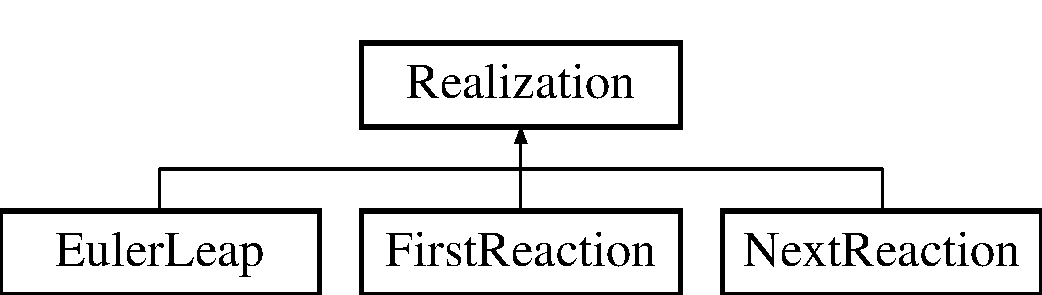
\includegraphics[height=2.000000cm]{class_realization}
\end{center}
\end{figure}
\subsection*{Public Member Functions}
\begin{DoxyCompactItemize}
\item 
\hyperlink{class_realization_af4cfb6f2221bef9ba5ad09564796677f}{Realization} (\hyperlink{class_model}{Model} $\ast$\hyperlink{class_realization_a47ec1d062b8caee874b08c1a17d6aeeb}{the\+\_\+model}, const \hyperlink{class_paramset}{Paramset} \&\hyperlink{class_realization_a119bb29de88929bc51bc1b329473a94b}{the\+\_\+paramset}, \hyperlink{classrng}{rng} $\ast$\hyperlink{class_realization_ac8d358d929afae90cf5790675b6744f9}{the\+\_\+rng}, int \hyperlink{class_realization_ad9951a0829e68e12fcb3817735bb5097}{n\+\_\+vars}, int \hyperlink{class_realization_afb711282bef806fc0020f91252d1df2c}{n\+\_\+events})
\begin{DoxyCompactList}\small\item\em Default constructor for \hyperlink{class_realization}{Realization}. \end{DoxyCompactList}\item 
virtual \hyperlink{class_realization_a040c39b39c5057c668bd264b4329f2b4}{$\sim$\+Realization} ()
\begin{DoxyCompactList}\small\item\em Destructor of \hyperlink{class_realization}{Realization}. \end{DoxyCompactList}\item 
int \hyperlink{class_realization_a4e21bc7355e33c17d1401736b3c62413}{simulate} (std\+::ofstream \&myfile)
\begin{DoxyCompactList}\small\item\em Simulates the realization from t\+\_\+inital to t\+\_\+final. \end{DoxyCompactList}\item 
\mbox{\Hypertarget{class_realization_a9949217117927b149850288f3b74c9ef}\label{class_realization_a9949217117927b149850288f3b74c9ef}} 
virtual int \hyperlink{class_realization_a9949217117927b149850288f3b74c9ef}{step} ()=0
\begin{DoxyCompactList}\small\item\em takes one simulation step according to the chosen algorithm \end{DoxyCompactList}\item 
bool \hyperlink{class_realization_a48953442ebf235cd1e02731c7419f65f}{rates\+\_\+are\+\_\+zero} ()
\begin{DoxyCompactList}\small\item\em checks whether all rates are zero \end{DoxyCompactList}\item 
int \hyperlink{class_realization_ab7ef90279eef4bf11261084f541c7bb0}{output\+\_\+state} (std\+::ofstream \&myfile)
\begin{DoxyCompactList}\small\item\em Prints the current state of the simulation. \end{DoxyCompactList}\item 
virtual int \hyperlink{class_realization_a391a89af7574a9053f53f8a299c2cc70}{set\+\_\+to\+\_\+initial\+\_\+state} ()
\begin{DoxyCompactList}\small\item\em Sets state\+\_\+array and state\+\_\+time to their user-\/specified initial values. \end{DoxyCompactList}\end{DoxyCompactItemize}
\subsection*{Public Attributes}
\begin{DoxyCompactItemize}
\item 
\mbox{\Hypertarget{class_realization_a47ec1d062b8caee874b08c1a17d6aeeb}\label{class_realization_a47ec1d062b8caee874b08c1a17d6aeeb}} 
\hyperlink{class_model}{Model} $\ast$ \hyperlink{class_realization_a47ec1d062b8caee874b08c1a17d6aeeb}{the\+\_\+model}
\begin{DoxyCompactList}\small\item\em the\+\_\+model is a \hyperlink{class_model}{Model} instance \end{DoxyCompactList}\item 
\mbox{\Hypertarget{class_realization_a119bb29de88929bc51bc1b329473a94b}\label{class_realization_a119bb29de88929bc51bc1b329473a94b}} 
const \hyperlink{class_paramset}{Paramset} \hyperlink{class_realization_a119bb29de88929bc51bc1b329473a94b}{the\+\_\+paramset}
\begin{DoxyCompactList}\small\item\em the\+\_\+paramset is a \hyperlink{class_paramset}{Paramset} instance \end{DoxyCompactList}\item 
\mbox{\Hypertarget{class_realization_ac8d358d929afae90cf5790675b6744f9}\label{class_realization_ac8d358d929afae90cf5790675b6744f9}} 
\hyperlink{classrng}{rng} $\ast$ \hyperlink{class_realization_ac8d358d929afae90cf5790675b6744f9}{the\+\_\+rng}
\begin{DoxyCompactList}\small\item\em the\+\_\+rng is an random number generator \end{DoxyCompactList}\item 
\mbox{\Hypertarget{class_realization_ad9951a0829e68e12fcb3817735bb5097}\label{class_realization_ad9951a0829e68e12fcb3817735bb5097}} 
const int \hyperlink{class_realization_ad9951a0829e68e12fcb3817735bb5097}{n\+\_\+vars}
\begin{DoxyCompactList}\small\item\em n\+\_\+vars is an int specifying number of variables \end{DoxyCompactList}\item 
\mbox{\Hypertarget{class_realization_afb711282bef806fc0020f91252d1df2c}\label{class_realization_afb711282bef806fc0020f91252d1df2c}} 
const int \hyperlink{class_realization_afb711282bef806fc0020f91252d1df2c}{n\+\_\+events}
\begin{DoxyCompactList}\small\item\em n\+\_\+events is an int specifying number of events \end{DoxyCompactList}\item 
\mbox{\Hypertarget{class_realization_a126f89978f0407873473222171333ee1}\label{class_realization_a126f89978f0407873473222171333ee1}} 
double $\ast$ \hyperlink{class_realization_a126f89978f0407873473222171333ee1}{state\+\_\+array}
\begin{DoxyCompactList}\small\item\em state\+\_\+array is a double array specifiying variable values of a function \end{DoxyCompactList}\item 
\mbox{\Hypertarget{class_realization_a9c52d8c6aa0ad99dbbec1e98302db7d8}\label{class_realization_a9c52d8c6aa0ad99dbbec1e98302db7d8}} 
double $\ast$ \hyperlink{class_realization_a9c52d8c6aa0ad99dbbec1e98302db7d8}{rates}
\begin{DoxyCompactList}\small\item\em rates is a double array specifying variable values of a rate function \end{DoxyCompactList}\item 
\mbox{\Hypertarget{class_realization_a7c4def45c4833072317517b71e723793}\label{class_realization_a7c4def45c4833072317517b71e723793}} 
double \hyperlink{class_realization_a7c4def45c4833072317517b71e723793}{state\+\_\+time}
\begin{DoxyCompactList}\small\item\em state\+\_\+time is a double that tracks state progress \end{DoxyCompactList}\end{DoxyCompactItemize}


\subsection{Detailed Description}
Class \hyperlink{class_realization}{Realization} holds realizations of a \hyperlink{class_model}{Model} (state array, propensities, waiting times, etc.) 

\subsection{Constructor \& Destructor Documentation}
\mbox{\Hypertarget{class_realization_af4cfb6f2221bef9ba5ad09564796677f}\label{class_realization_af4cfb6f2221bef9ba5ad09564796677f}} 
\index{Realization@{Realization}!Realization@{Realization}}
\index{Realization@{Realization}!Realization@{Realization}}
\subsubsection{\texorpdfstring{Realization()}{Realization()}}
{\footnotesize\ttfamily Realization\+::\+Realization (\begin{DoxyParamCaption}\item[{\hyperlink{class_model}{Model} $\ast$}]{the\+\_\+model,  }\item[{const \hyperlink{class_paramset}{Paramset} \&}]{the\+\_\+paramset,  }\item[{\hyperlink{classrng}{rng} $\ast$}]{the\+\_\+rng,  }\item[{int}]{n\+\_\+vars,  }\item[{int}]{n\+\_\+events }\end{DoxyParamCaption})}



Default constructor for \hyperlink{class_realization}{Realization}. 


\begin{DoxyParams}{Parameters}
{\em the\+\_\+model} & is a \hyperlink{class_model}{Model} object \\
\hline
{\em the\+\_\+paramset} & is a \hyperlink{class_paramset}{Paramset} object \\
\hline
{\em the\+\_\+rng} & is a random number generator \\
\hline
{\em n\+\_\+vars} & is an int specifying variable count \\
\hline
{\em n\+\_\+events} & is an int specifying event count\\
\hline
\end{DoxyParams}
\begin{DoxyReturn}{Returns}
nothing 
\end{DoxyReturn}
\mbox{\Hypertarget{class_realization_a040c39b39c5057c668bd264b4329f2b4}\label{class_realization_a040c39b39c5057c668bd264b4329f2b4}} 
\index{Realization@{Realization}!````~Realization@{$\sim$\+Realization}}
\index{````~Realization@{$\sim$\+Realization}!Realization@{Realization}}
\subsubsection{\texorpdfstring{$\sim$\+Realization()}{~Realization()}}
{\footnotesize\ttfamily Realization\+::$\sim$\+Realization (\begin{DoxyParamCaption}{ }\end{DoxyParamCaption})\hspace{0.3cm}{\ttfamily [virtual]}}



Destructor of \hyperlink{class_realization}{Realization}. 

\begin{DoxyReturn}{Returns}
nothing 
\end{DoxyReturn}


\subsection{Member Function Documentation}
\mbox{\Hypertarget{class_realization_ab7ef90279eef4bf11261084f541c7bb0}\label{class_realization_ab7ef90279eef4bf11261084f541c7bb0}} 
\index{Realization@{Realization}!output\+\_\+state@{output\+\_\+state}}
\index{output\+\_\+state@{output\+\_\+state}!Realization@{Realization}}
\subsubsection{\texorpdfstring{output\+\_\+state()}{output\_state()}}
{\footnotesize\ttfamily int Realization\+::output\+\_\+state (\begin{DoxyParamCaption}\item[{std\+::ofstream \&}]{myfile }\end{DoxyParamCaption})}



Prints the current state of the simulation. 

\begin{DoxyReturn}{Returns}
int 
\end{DoxyReturn}
\mbox{\Hypertarget{class_realization_a48953442ebf235cd1e02731c7419f65f}\label{class_realization_a48953442ebf235cd1e02731c7419f65f}} 
\index{Realization@{Realization}!rates\+\_\+are\+\_\+zero@{rates\+\_\+are\+\_\+zero}}
\index{rates\+\_\+are\+\_\+zero@{rates\+\_\+are\+\_\+zero}!Realization@{Realization}}
\subsubsection{\texorpdfstring{rates\+\_\+are\+\_\+zero()}{rates\_are\_zero()}}
{\footnotesize\ttfamily bool Realization\+::rates\+\_\+are\+\_\+zero (\begin{DoxyParamCaption}{ }\end{DoxyParamCaption})}



checks whether all rates are zero 

\begin{DoxyReturn}{Returns}
bool 
\end{DoxyReturn}
\mbox{\Hypertarget{class_realization_a391a89af7574a9053f53f8a299c2cc70}\label{class_realization_a391a89af7574a9053f53f8a299c2cc70}} 
\index{Realization@{Realization}!set\+\_\+to\+\_\+initial\+\_\+state@{set\+\_\+to\+\_\+initial\+\_\+state}}
\index{set\+\_\+to\+\_\+initial\+\_\+state@{set\+\_\+to\+\_\+initial\+\_\+state}!Realization@{Realization}}
\subsubsection{\texorpdfstring{set\+\_\+to\+\_\+initial\+\_\+state()}{set\_to\_initial\_state()}}
{\footnotesize\ttfamily int Realization\+::set\+\_\+to\+\_\+initial\+\_\+state (\begin{DoxyParamCaption}{ }\end{DoxyParamCaption})\hspace{0.3cm}{\ttfamily [virtual]}}



Sets state\+\_\+array and state\+\_\+time to their user-\/specified initial values. 

\begin{DoxyReturn}{Returns}
int 
\end{DoxyReturn}


Reimplemented in \hyperlink{class_euler_leap_a1a13929ea1ebf40e7357439968828f4b}{Euler\+Leap}, \hyperlink{class_midpoint_leap_a177682cf5042407ccee1a443e8920896}{Midpoint\+Leap}, and \hyperlink{class_next_reaction_a0cc63c4ec9fe3f338472fff302f6d746}{Next\+Reaction}.

\mbox{\Hypertarget{class_realization_a4e21bc7355e33c17d1401736b3c62413}\label{class_realization_a4e21bc7355e33c17d1401736b3c62413}} 
\index{Realization@{Realization}!simulate@{simulate}}
\index{simulate@{simulate}!Realization@{Realization}}
\subsubsection{\texorpdfstring{simulate()}{simulate()}}
{\footnotesize\ttfamily int Realization\+::simulate (\begin{DoxyParamCaption}\item[{std\+::ofstream \&}]{myfile }\end{DoxyParamCaption})}



Simulates the realization from t\+\_\+inital to t\+\_\+final. 

\begin{DoxyReturn}{Returns}
int 
\end{DoxyReturn}


The documentation for this class was generated from the following files\+:\begin{DoxyCompactItemize}
\item 
/\+Users/\+Caleb/\+A\+P\+C524/stoched/src/\hyperlink{realization_8h}{realization.\+h}\item 
/\+Users/\+Caleb/\+A\+P\+C524/stoched/src/\hyperlink{realization_8cc}{realization.\+cc}\end{DoxyCompactItemize}

\hypertarget{class_realization_factory}{}\section{Realization\+Factory Class Reference}
\label{class_realization_factory}\index{Realization\+Factory@{Realization\+Factory}}


Class \hyperlink{class_realization_factory}{Realization\+Factory} generates required instance of \hyperlink{class_realization}{Realization} (\hyperlink{class_first_reaction}{First\+Reaction}, \hyperlink{class_next_reaction}{Next\+Reaction}, \hyperlink{class_euler_leap}{Euler\+Leap}) based on input.  




{\ttfamily \#include $<$realization\+\_\+factory.\+h$>$}

\subsection*{Static Public Member Functions}
\begin{DoxyCompactItemize}
\item 
static \hyperlink{class_realization}{Realization} $\ast$ \hyperlink{class_realization_factory_a4881816e453d1107de053ea3c0b8d8ba}{New\+Realization} (\hyperlink{class_model}{Model} $\ast$the\+\_\+model, const \hyperlink{class_paramset}{Paramset} \&the\+\_\+paramset, \hyperlink{classrng}{rng} $\ast$the\+\_\+rng, int n\+\_\+vars, int n\+\_\+events)
\begin{DoxyCompactList}\small\item\em Create new realization. \end{DoxyCompactList}\end{DoxyCompactItemize}


\subsection{Detailed Description}
Class \hyperlink{class_realization_factory}{Realization\+Factory} generates required instance of \hyperlink{class_realization}{Realization} (\hyperlink{class_first_reaction}{First\+Reaction}, \hyperlink{class_next_reaction}{Next\+Reaction}, \hyperlink{class_euler_leap}{Euler\+Leap}) based on input. 

\subsection{Member Function Documentation}
\mbox{\Hypertarget{class_realization_factory_a4881816e453d1107de053ea3c0b8d8ba}\label{class_realization_factory_a4881816e453d1107de053ea3c0b8d8ba}} 
\index{Realization\+Factory@{Realization\+Factory}!New\+Realization@{New\+Realization}}
\index{New\+Realization@{New\+Realization}!Realization\+Factory@{Realization\+Factory}}
\subsubsection{\texorpdfstring{New\+Realization()}{NewRealization()}}
{\footnotesize\ttfamily \hyperlink{class_realization}{Realization} $\ast$ Realization\+Factory\+::\+New\+Realization (\begin{DoxyParamCaption}\item[{\hyperlink{class_model}{Model} $\ast$}]{the\+\_\+model,  }\item[{const \hyperlink{class_paramset}{Paramset} \&}]{the\+\_\+paramset,  }\item[{\hyperlink{classrng}{rng} $\ast$}]{the\+\_\+rng,  }\item[{int}]{n\+\_\+vars,  }\item[{int}]{n\+\_\+events }\end{DoxyParamCaption})\hspace{0.3cm}{\ttfamily [static]}}



Create new realization. 


\begin{DoxyParams}{Parameters}
{\em the\+\_\+model} & is a \hyperlink{class_model}{Model} object \\
\hline
{\em the\+\_\+paramset} & is a \hyperlink{class_paramset}{Paramset} object \\
\hline
{\em the\+\_\+rng} & is a random number generator \\
\hline
{\em n\+\_\+vars} & is an int specifying variable count \\
\hline
{\em n\+\_\+events} & is an int specifying event count\\
\hline
\end{DoxyParams}
\begin{DoxyReturn}{Returns}
nothing 
\end{DoxyReturn}


The documentation for this class was generated from the following files\+:\begin{DoxyCompactItemize}
\item 
/\+Users/dylan/stoched/src/\hyperlink{realization__factory_8h}{realization\+\_\+factory.\+h}\item 
/\+Users/dylan/stoched/src/\hyperlink{realization__factory_8cc}{realization\+\_\+factory.\+cc}\end{DoxyCompactItemize}

\hypertarget{classrng}{}\section{rng Class Reference}
\label{classrng}\index{rng@{rng}}


Class rng implements random number generator, based upon public domain xorshift implementations by David Blackman and Sebastiano Vigna (\href{mailto:vigna@acm.org}{\tt vigna@acm.\+org})  




{\ttfamily \#include $<$rng.\+h$>$}

Inheritance diagram for rng\+:\begin{figure}[H]
\begin{center}
\leavevmode
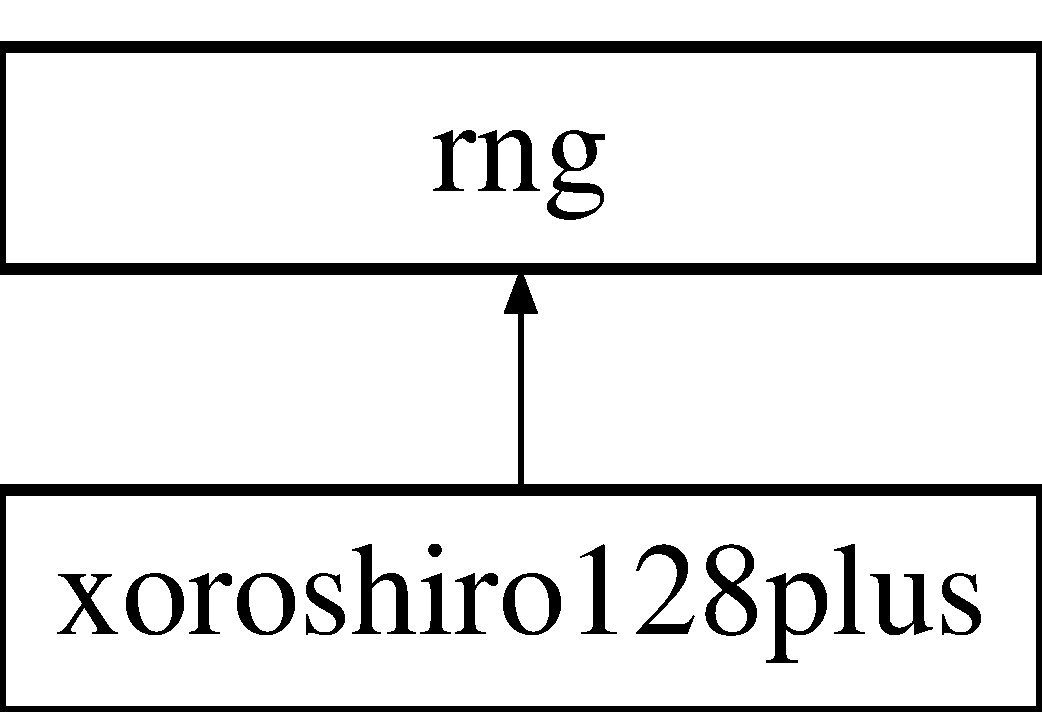
\includegraphics[height=2.000000cm]{classrng}
\end{center}
\end{figure}
\subsection*{Public Member Functions}
\begin{DoxyCompactItemize}
\item 
\mbox{\Hypertarget{classrng_acc0ef5e0bf2bee28c37070ddb4c21175}\label{classrng_acc0ef5e0bf2bee28c37070ddb4c21175}} 
virtual \hyperlink{classrng_acc0ef5e0bf2bee28c37070ddb4c21175}{$\sim$rng} ()
\begin{DoxyCompactList}\small\item\em Destructor of rng object. \end{DoxyCompactList}\item 
\mbox{\Hypertarget{classrng_a0fa7d2415b07e3396b6ed3fb7c238606}\label{classrng_a0fa7d2415b07e3396b6ed3fb7c238606}} 
virtual uint64\+\_\+t \hyperlink{classrng_a0fa7d2415b07e3396b6ed3fb7c238606}{next} ()=0
\begin{DoxyCompactList}\small\item\em get a new random int64 \end{DoxyCompactList}\item 
\mbox{\Hypertarget{classrng_a3f0fec3ad9a286726825fddbf78aada8}\label{classrng_a3f0fec3ad9a286726825fddbf78aada8}} 
virtual double \hyperlink{classrng_a3f0fec3ad9a286726825fddbf78aada8}{runif} ()=0
\begin{DoxyCompactList}\small\item\em get a new random uniform(0, 1) RV \end{DoxyCompactList}\item 
\mbox{\Hypertarget{classrng_a7770e4ceae3bad5c426784b4b2148a1d}\label{classrng_a7770e4ceae3bad5c426784b4b2148a1d}} 
double \hyperlink{classrng_a7770e4ceae3bad5c426784b4b2148a1d}{rexp} (double lambda)
\begin{DoxyCompactList}\small\item\em get a new random exponential(lambda) RV \end{DoxyCompactList}\item 
\mbox{\Hypertarget{classrng_a9c16bdeae3be90e8bd30eb284a4b2980}\label{classrng_a9c16bdeae3be90e8bd30eb284a4b2980}} 
long \hyperlink{classrng_a9c16bdeae3be90e8bd30eb284a4b2980}{rpois} (double mean)
\begin{DoxyCompactList}\small\item\em get a new random poisson(mean) RV \end{DoxyCompactList}\item 
\mbox{\Hypertarget{classrng_a2203fb1d2504c000306be5a0035d1a6c}\label{classrng_a2203fb1d2504c000306be5a0035d1a6c}} 
virtual void \hyperlink{classrng_a2203fb1d2504c000306be5a0035d1a6c}{jump} ()=0
\begin{DoxyCompactList}\small\item\em quick 2$^\wedge$64 calls to next (for parallelism) \end{DoxyCompactList}\item 
double \hyperlink{classrng_ae85750e7f1befc4d1016731248dd3e80}{log\+\_\+factorial} (int k)
\end{DoxyCompactItemize}
\subsection*{Private Member Functions}
\begin{DoxyCompactItemize}
\item 
\mbox{\Hypertarget{classrng_a1fd45ffcc5dc65bdf23311f97fd0630c}\label{classrng_a1fd45ffcc5dc65bdf23311f97fd0630c}} 
long \hyperlink{classrng_a1fd45ffcc5dc65bdf23311f97fd0630c}{poisson\+\_\+knuth} (double mean)
\begin{DoxyCompactList}\small\item\em random poisson \end{DoxyCompactList}\item 
\mbox{\Hypertarget{classrng_aefbbe59c0bb810de0337855e77b36747}\label{classrng_aefbbe59c0bb810de0337855e77b36747}} 
long \hyperlink{classrng_aefbbe59c0bb810de0337855e77b36747}{poisson\+\_\+ptrs} (double mean)
\begin{DoxyCompactList}\small\item\em random poisson \end{DoxyCompactList}\end{DoxyCompactItemize}


\subsection{Detailed Description}
Class rng implements random number generator, based upon public domain xorshift implementations by David Blackman and Sebastiano Vigna (\href{mailto:vigna@acm.org}{\tt vigna@acm.\+org}) 

\subsection{Member Function Documentation}
\mbox{\Hypertarget{classrng_ae85750e7f1befc4d1016731248dd3e80}\label{classrng_ae85750e7f1befc4d1016731248dd3e80}} 
\index{rng@{rng}!log\+\_\+factorial@{log\+\_\+factorial}}
\index{log\+\_\+factorial@{log\+\_\+factorial}!rng@{rng}}
\subsubsection{\texorpdfstring{log\+\_\+factorial()}{log\_factorial()}}
{\footnotesize\ttfamily double rng\+::log\+\_\+factorial (\begin{DoxyParamCaption}\item[{int}]{k }\end{DoxyParamCaption})}

log factorial function modified from public domain C\# implementation by John D. Cook (\href{http://www.johndcook.com/blog/csharp_log_factorial/}{\tt http\+://www.\+johndcook.\+com/blog/csharp\+\_\+log\+\_\+factorial/}) and P\+T\+RS algorithm by Wolfgang Hoermann (1993) 

The documentation for this class was generated from the following files\+:\begin{DoxyCompactItemize}
\item 
/\+Users/\+Caleb/\+A\+P\+C524/stoched/src/\hyperlink{rng_8h}{rng.\+h}\item 
/\+Users/\+Caleb/\+A\+P\+C524/stoched/src/\hyperlink{rng_8cc}{rng.\+cc}\end{DoxyCompactItemize}

\hypertarget{classxoroshiro128plus}{}\section{xoroshiro128plus Class Reference}
\label{classxoroshiro128plus}\index{xoroshiro128plus@{xoroshiro128plus}}


Class \hyperlink{classxoroshiro128plus}{xoroshiro128plus} implements a random number generator of Class rng.  




{\ttfamily \#include $<$xoroshiro128plus.\+h$>$}

Inheritance diagram for xoroshiro128plus\+:\begin{figure}[H]
\begin{center}
\leavevmode
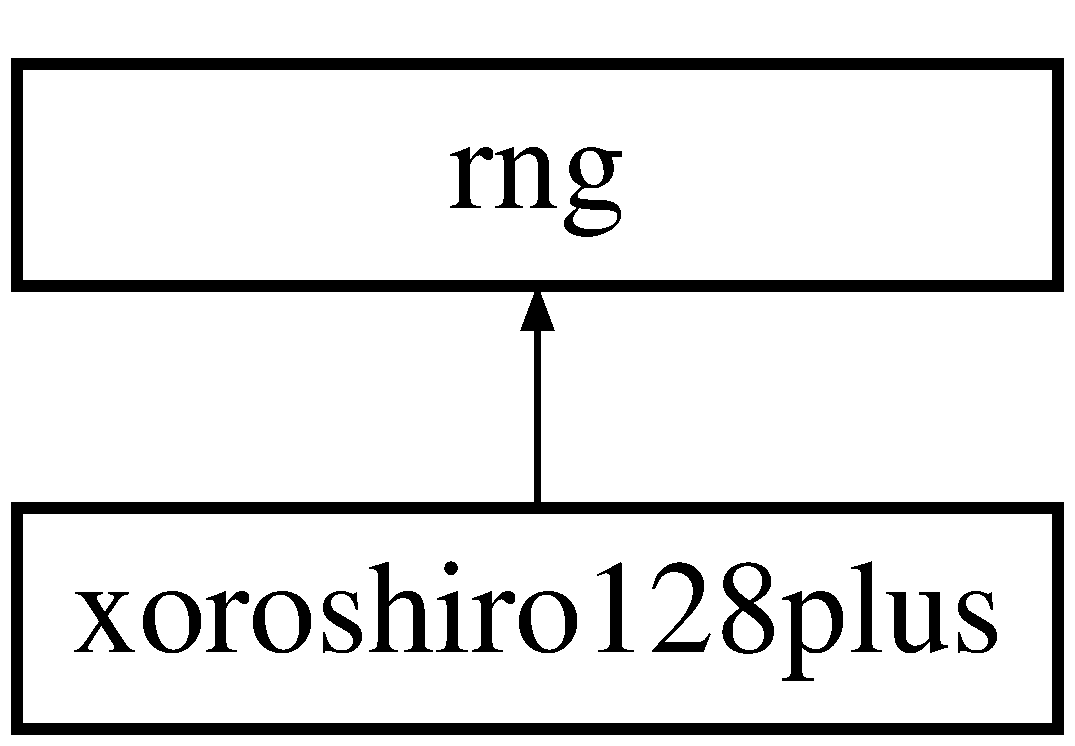
\includegraphics[height=2.000000cm]{classxoroshiro128plus}
\end{center}
\end{figure}
\subsection*{Public Member Functions}
\begin{DoxyCompactItemize}
\item 
\hyperlink{classxoroshiro128plus_ae32867bf0900c675d3b6f638ea2c49e1}{xoroshiro128plus} (int seed)
\begin{DoxyCompactList}\small\item\em Default constructor. \end{DoxyCompactList}\item 
\mbox{\Hypertarget{classxoroshiro128plus_ae6dfa2376788f9632175a385c6cf74ef}\label{classxoroshiro128plus_ae6dfa2376788f9632175a385c6cf74ef}} 
\hyperlink{classxoroshiro128plus_ae6dfa2376788f9632175a385c6cf74ef}{$\sim$xoroshiro128plus} ()
\begin{DoxyCompactList}\small\item\em Default Destructor for Xoroshiro128plus. \end{DoxyCompactList}\item 
\mbox{\Hypertarget{classxoroshiro128plus_a14185bcb657d561663803f4a8b2e9a92}\label{classxoroshiro128plus_a14185bcb657d561663803f4a8b2e9a92}} 
uint64\+\_\+t \hyperlink{classxoroshiro128plus_a14185bcb657d561663803f4a8b2e9a92}{next} ()
\begin{DoxyCompactList}\small\item\em get random int and update state \end{DoxyCompactList}\item 
\mbox{\Hypertarget{classxoroshiro128plus_a5054e4de9c05fdab89ab41dbfe05a424}\label{classxoroshiro128plus_a5054e4de9c05fdab89ab41dbfe05a424}} 
double \hyperlink{classxoroshiro128plus_a5054e4de9c05fdab89ab41dbfe05a424}{runif} ()
\begin{DoxyCompactList}\small\item\em get random uniform(0, 1) double and update state \end{DoxyCompactList}\item 
void \hyperlink{classxoroshiro128plus_a8058dee37dfc67409ed8674ba8f830a9}{jump} ()
\end{DoxyCompactItemize}
\subsection*{Private Member Functions}
\begin{DoxyCompactItemize}
\item 
\mbox{\Hypertarget{classxoroshiro128plus_ac80afbdcbf2c512310c4aebe42f936f0}\label{classxoroshiro128plus_ac80afbdcbf2c512310c4aebe42f936f0}} 
uint64\+\_\+t \hyperlink{classxoroshiro128plus_ac80afbdcbf2c512310c4aebe42f936f0}{rotl} (const uint64\+\_\+t x, int k)
\begin{DoxyCompactList}\small\item\em simulated rotate \end{DoxyCompactList}\item 
\mbox{\Hypertarget{classxoroshiro128plus_aee8ea766a36b82e20c5fdc2c5184a41c}\label{classxoroshiro128plus_aee8ea766a36b82e20c5fdc2c5184a41c}} 
uint64\+\_\+t \hyperlink{classxoroshiro128plus_aee8ea766a36b82e20c5fdc2c5184a41c}{splitmix64} ()
\begin{DoxyCompactList}\small\item\em splitmix64 next function, for initializing generator \end{DoxyCompactList}\end{DoxyCompactItemize}
\subsection*{Private Attributes}
\begin{DoxyCompactItemize}
\item 
\mbox{\Hypertarget{classxoroshiro128plus_a50f3b4f14b1a5b3034d4cf3e6dde2b10}\label{classxoroshiro128plus_a50f3b4f14b1a5b3034d4cf3e6dde2b10}} 
uint64\+\_\+t {\bfseries s} \mbox{[}2\mbox{]}
\item 
\mbox{\Hypertarget{classxoroshiro128plus_acdcc17b31842b463c1a00360b182b3aa}\label{classxoroshiro128plus_acdcc17b31842b463c1a00360b182b3aa}} 
uint64\+\_\+t {\bfseries splitmixstate}
\end{DoxyCompactItemize}


\subsection{Detailed Description}
Class \hyperlink{classxoroshiro128plus}{xoroshiro128plus} implements a random number generator of Class rng. 

\subsection{Constructor \& Destructor Documentation}
\mbox{\Hypertarget{classxoroshiro128plus_ae32867bf0900c675d3b6f638ea2c49e1}\label{classxoroshiro128plus_ae32867bf0900c675d3b6f638ea2c49e1}} 
\index{xoroshiro128plus@{xoroshiro128plus}!xoroshiro128plus@{xoroshiro128plus}}
\index{xoroshiro128plus@{xoroshiro128plus}!xoroshiro128plus@{xoroshiro128plus}}
\subsubsection{\texorpdfstring{xoroshiro128plus()}{xoroshiro128plus()}}
{\footnotesize\ttfamily xoroshiro128plus\+::xoroshiro128plus (\begin{DoxyParamCaption}\item[{int}]{seed }\end{DoxyParamCaption})}



Default constructor. 

initialize state with splitmix64 random ints from seed int (prevents similar seeds from generating correlated states) 

\subsection{Member Function Documentation}
\mbox{\Hypertarget{classxoroshiro128plus_a8058dee37dfc67409ed8674ba8f830a9}\label{classxoroshiro128plus_a8058dee37dfc67409ed8674ba8f830a9}} 
\index{xoroshiro128plus@{xoroshiro128plus}!jump@{jump}}
\index{jump@{jump}!xoroshiro128plus@{xoroshiro128plus}}
\subsubsection{\texorpdfstring{jump()}{jump()}}
{\footnotesize\ttfamily void xoroshiro128plus\+::jump (\begin{DoxyParamCaption}{ }\end{DoxyParamCaption})\hspace{0.3cm}{\ttfamily [virtual]}}

This is the jump function for the generator. It is equivalent to 2$^\wedge$64 calls to \hyperlink{classxoroshiro128plus_a14185bcb657d561663803f4a8b2e9a92}{next()}; it can be used to generate 2$^\wedge$64 non-\/overlapping subsequences for parallel computations. 

Implements \hyperlink{classrng_a2203fb1d2504c000306be5a0035d1a6c}{rng}.



The documentation for this class was generated from the following files\+:\begin{DoxyCompactItemize}
\item 
/\+Users/dylan/stoched/src/\hyperlink{xoroshiro128plus_8h}{xoroshiro128plus.\+h}\item 
/\+Users/dylan/stoched/src/\hyperlink{xoroshiro128plus_8cc}{xoroshiro128plus.\+cc}\end{DoxyCompactItemize}

\chapter{File Documentation}
\hypertarget{eulerleap_8cc}{}\section{/\+Users/\+Caleb/\+A\+P\+C524/stoched/src/eulerleap.cc File Reference}
\label{eulerleap_8cc}\index{/\+Users/\+Caleb/\+A\+P\+C524/stoched/src/eulerleap.\+cc@{/\+Users/\+Caleb/\+A\+P\+C524/stoched/src/eulerleap.\+cc}}


Class \hyperlink{class_euler_leap}{Euler\+Leap} implements \hyperlink{class_realization}{Realization} step() function using Euler Leap method.  


{\ttfamily \#include \char`\"{}eulerleap.\+h\char`\"{}}\newline


\subsection{Detailed Description}
Class \hyperlink{class_euler_leap}{Euler\+Leap} implements \hyperlink{class_realization}{Realization} step() function using Euler Leap method. 

\begin{DoxyAuthor}{Author}
Dylan Morris (\href{mailto:dhmorris@princeton.edu}{\tt dhmorris@princeton.\+edu}) 
\end{DoxyAuthor}
\begin{DoxyDate}{Date}
12/6/16 
\end{DoxyDate}
\begin{DoxyVersion}{Version}
1.\+0 
\end{DoxyVersion}

\hypertarget{eulerleap_8h}{}\section{/\+Users/\+Caleb/\+A\+P\+C524/stoched/src/eulerleap.h File Reference}
\label{eulerleap_8h}\index{/\+Users/\+Caleb/\+A\+P\+C524/stoched/src/eulerleap.\+h@{/\+Users/\+Caleb/\+A\+P\+C524/stoched/src/eulerleap.\+h}}


Class \hyperlink{class_euler_leap}{Euler\+Leap} implements \hyperlink{class_realization}{Realization} step() function using Euler Leap method.  


{\ttfamily \#include \char`\"{}realization.\+h\char`\"{}}\newline
{\ttfamily \#include $<$stdexcept$>$}\newline
\subsection*{Classes}
\begin{DoxyCompactItemize}
\item 
class \hyperlink{class_euler_leap}{Euler\+Leap}
\begin{DoxyCompactList}\small\item\em Class \hyperlink{class_euler_leap}{Euler\+Leap} implements \hyperlink{class_realization}{Realization} step() function using Euler Leap method. \end{DoxyCompactList}\end{DoxyCompactItemize}


\subsection{Detailed Description}
Class \hyperlink{class_euler_leap}{Euler\+Leap} implements \hyperlink{class_realization}{Realization} step() function using Euler Leap method. 

\begin{DoxyAuthor}{Author}
Dylan Morris (\href{mailto:dhmorris@princeton.edu}{\tt dhmorris@princeton.\+edu}) 
\end{DoxyAuthor}
\begin{DoxyDate}{Date}
12/6/16 
\end{DoxyDate}
\begin{DoxyVersion}{Version}
1.\+0 
\end{DoxyVersion}

\hypertarget{event_8cc}{}\section{/\+Users/\+Caleb/\+A\+P\+C524/stoched/src/event.cc File Reference}
\label{event_8cc}\index{/\+Users/\+Caleb/\+A\+P\+C524/stoched/src/event.\+cc@{/\+Users/\+Caleb/\+A\+P\+C524/stoched/src/event.\+cc}}


A\+PC 524, Final Project -\/ Stoched.  


{\ttfamily \#include \char`\"{}event.\+h\char`\"{}}\newline
{\ttfamily \#include \char`\"{}fparser/fparser.\+hh\char`\"{}}\newline
{\ttfamily \#include $<$assert.\+h$>$}\newline
{\ttfamily \#include $<$stdio.\+h$>$}\newline
{\ttfamily \#include $<$iostream$>$}\newline


\subsection{Detailed Description}
A\+PC 524, Final Project -\/ Stoched. 

\begin{DoxyAuthor}{Author}
Caleb Peckham (\href{mailto:peckham@princeton.edu}{\tt peckham@princeton.\+edu}) 
\end{DoxyAuthor}
\begin{DoxyDate}{Date}
12/6/16 
\end{DoxyDate}
\begin{DoxyVersion}{Version}
1.\+0
\end{DoxyVersion}
\hypertarget{event.cc_DESCRIPTION}{}\subsection{D\+E\+S\+C\+R\+I\+P\+T\+I\+ON}\label{event.cc_DESCRIPTION}

\hypertarget{event_8h}{}\section{/\+Users/dylan/stoched/src/event.h File Reference}
\label{event_8h}\index{/\+Users/dylan/stoched/src/event.\+h@{/\+Users/dylan/stoched/src/event.\+h}}


Class \hyperlink{class_event}{Event} holds a user-\/specified event, namely set of functions and associated rate.  


{\ttfamily \#include \char`\"{}fparser/fparser.\+hh\char`\"{}}\newline
\subsection*{Classes}
\begin{DoxyCompactItemize}
\item 
class \hyperlink{class_event}{Event}
\begin{DoxyCompactList}\small\item\em Class \hyperlink{class_event}{Event} holds a user-\/specified event, namely set of functions and associated rate. \end{DoxyCompactList}\end{DoxyCompactItemize}


\subsection{Detailed Description}
Class \hyperlink{class_event}{Event} holds a user-\/specified event, namely set of functions and associated rate. 

\begin{DoxyAuthor}{Author}
Caleb Peckham (\href{mailto:peckham@princeton.edu}{\tt peckham@princeton.\+edu}) 
\end{DoxyAuthor}
\begin{DoxyDate}{Date}
12/6/16 
\end{DoxyDate}
\begin{DoxyVersion}{Version}
1.\+0 
\end{DoxyVersion}

\hypertarget{eventtests_8cc}{}\section{/\+Users/\+Caleb/\+A\+P\+C524/stoched/src/eventtests.cc File Reference}
\label{eventtests_8cc}\index{/\+Users/\+Caleb/\+A\+P\+C524/stoched/src/eventtests.\+cc@{/\+Users/\+Caleb/\+A\+P\+C524/stoched/src/eventtests.\+cc}}


Test \hyperlink{class_event}{Event} code.  


{\ttfamily \#include $<$string$>$}\newline
{\ttfamily \#include $<$stdio.\+h$>$}\newline
{\ttfamily \#include $<$iostream$>$}\newline
{\ttfamily \#include \char`\"{}event.\+h\char`\"{}}\newline
{\ttfamily \#include \char`\"{}gtest/gtest.\+h\char`\"{}}\newline
\subsection*{Functions}
\begin{DoxyCompactItemize}
\item 
\mbox{\Hypertarget{eventtests_8cc_a6b161b8adf7b6aedd391ff50ef4aab48}\label{eventtests_8cc_a6b161b8adf7b6aedd391ff50ef4aab48}} 
{\bfseries T\+E\+S\+T\+\_\+F} (Event\+Tests, Use\+Function)
\item 
\mbox{\Hypertarget{eventtests_8cc_aef21222dcf46efeb336bc7e75f85b13b}\label{eventtests_8cc_aef21222dcf46efeb336bc7e75f85b13b}} 
{\bfseries T\+E\+S\+T\+\_\+F} (Event\+Tests, Rate\+Function)
\item 
\mbox{\Hypertarget{eventtests_8cc_a3c04138a5bfe5d72780bb7e82a18e627}\label{eventtests_8cc_a3c04138a5bfe5d72780bb7e82a18e627}} 
int {\bfseries main} (int argc, char $\ast$$\ast$argv)
\end{DoxyCompactItemize}


\subsection{Detailed Description}
Test \hyperlink{class_event}{Event} code. 

\begin{DoxyAuthor}{Author}
Caleb Peckham (\href{mailto:peckham@princeton.edu}{\tt peckham@princeton.\+edu}) 
\end{DoxyAuthor}
\begin{DoxyDate}{Date}
1/12/17 
\end{DoxyDate}
\begin{DoxyVersion}{Version}
1.\+0 
\end{DoxyVersion}

\hypertarget{firstreaction_8cc}{}\section{/\+Users/\+Caleb/\+A\+P\+C524/stoched/src/firstreaction.cc File Reference}
\label{firstreaction_8cc}\index{/\+Users/\+Caleb/\+A\+P\+C524/stoched/src/firstreaction.\+cc@{/\+Users/\+Caleb/\+A\+P\+C524/stoched/src/firstreaction.\+cc}}


Inherit \hyperlink{class_realization}{Realization} class for first reaction instance.  


{\ttfamily \#include \char`\"{}firstreaction.\+h\char`\"{}}\newline


\subsection{Detailed Description}
Inherit \hyperlink{class_realization}{Realization} class for first reaction instance. 

Inherit \hyperlink{class_realization}{Realization} class for next reaction instance.

\begin{DoxyAuthor}{Author}
Dylan Morris (\href{mailto:dhmorris@princeton.edu}{\tt dhmorris@princeton.\+edu}) 
\end{DoxyAuthor}
\begin{DoxyDate}{Date}
12/6/16 
\end{DoxyDate}
\begin{DoxyVersion}{Version}
1.\+0 
\end{DoxyVersion}

\hypertarget{firstreaction_8h}{}\section{/\+Users/\+Caleb/\+A\+P\+C524/stoched/src/firstreaction.h File Reference}
\label{firstreaction_8h}\index{/\+Users/\+Caleb/\+A\+P\+C524/stoched/src/firstreaction.\+h@{/\+Users/\+Caleb/\+A\+P\+C524/stoched/src/firstreaction.\+h}}


Class \hyperlink{class_first_reaction}{First\+Reaction} implements \hyperlink{class_realization}{Realization} step() function using the exact First Reaction algorithm of Gillespie (1971)  


{\ttfamily \#include \char`\"{}realization.\+h\char`\"{}}\newline
\subsection*{Classes}
\begin{DoxyCompactItemize}
\item 
class \hyperlink{class_first_reaction}{First\+Reaction}
\begin{DoxyCompactList}\small\item\em Class \hyperlink{class_first_reaction}{First\+Reaction} implements \hyperlink{class_realization}{Realization} \hyperlink{class_first_reaction_aed63c3c95d20b2ad557dabb6c5376a73}{step()} function using the exact First Reaction algorithm of Gillespie (1971) \end{DoxyCompactList}\end{DoxyCompactItemize}


\subsection{Detailed Description}
Class \hyperlink{class_first_reaction}{First\+Reaction} implements \hyperlink{class_realization}{Realization} step() function using the exact First Reaction algorithm of Gillespie (1971) 

\begin{DoxyAuthor}{Author}
Dylan Morris (\href{mailto:dhmorris@princeton.edu}{\tt dhmorris@princeton.\+edu}) 
\end{DoxyAuthor}
\begin{DoxyDate}{Date}
12/6/16 
\end{DoxyDate}
\begin{DoxyVersion}{Version}
1.\+0 
\end{DoxyVersion}

\hypertarget{midpointleap_8cc}{}\section{/\+Users/dylan/stoched/src/midpointleap.cc File Reference}
\label{midpointleap_8cc}\index{/\+Users/dylan/stoched/src/midpointleap.\+cc@{/\+Users/dylan/stoched/src/midpointleap.\+cc}}


Class \hyperlink{class_midpoint_leap}{Midpoint\+Leap} implements \hyperlink{class_realization}{Realization} step() function using the midpoint tau leap approximate algorithm of Gillepsie (2001). The method is analogous to the deterministic midpoint (2nd-\/order Runge-\/\+Kutta) method for the numerical solution of ordinary differential equations.  


{\ttfamily \#include \char`\"{}midpointleap.\+h\char`\"{}}\newline


\subsection{Detailed Description}
Class \hyperlink{class_midpoint_leap}{Midpoint\+Leap} implements \hyperlink{class_realization}{Realization} step() function using the midpoint tau leap approximate algorithm of Gillepsie (2001). The method is analogous to the deterministic midpoint (2nd-\/order Runge-\/\+Kutta) method for the numerical solution of ordinary differential equations. 

\begin{DoxyAuthor}{Author}
Dylan Morris (\href{mailto:dhmorris@princeton.edu}{\tt dhmorris@princeton.\+edu}) 
\end{DoxyAuthor}
\begin{DoxyDate}{Date}
2016-\/01-\/16 
\end{DoxyDate}
\begin{DoxyVersion}{Version}
1.\+0 
\end{DoxyVersion}

\hypertarget{midpointleap_8h}{}\section{/\+Users/\+Caleb/\+A\+P\+C524/stoched/src/midpointleap.h File Reference}
\label{midpointleap_8h}\index{/\+Users/\+Caleb/\+A\+P\+C524/stoched/src/midpointleap.\+h@{/\+Users/\+Caleb/\+A\+P\+C524/stoched/src/midpointleap.\+h}}


Class \hyperlink{class_midpoint_leap}{Midpoint\+Leap} implements \hyperlink{class_realization}{Realization} step() function using the midpoint tau leap approximate algorithm of Gillepsie (2001). The method is analogous to the deterministic midpoint (2nd-\/order Runge-\/\+Kutta) method for the numerical solution of ordinary differential equations.  


{\ttfamily \#include $<$stdexcept$>$}\newline
{\ttfamily \#include \char`\"{}realization.\+h\char`\"{}}\newline
\subsection*{Classes}
\begin{DoxyCompactItemize}
\item 
class \hyperlink{class_midpoint_leap}{Midpoint\+Leap}
\begin{DoxyCompactList}\small\item\em Class \hyperlink{class_midpoint_leap}{Midpoint\+Leap} implements \hyperlink{class_realization}{Realization} \hyperlink{class_midpoint_leap_a8afc1a6a8777157f7b42ec08a848b564}{step()} function using the midpoint tau leap approximate algorithm of Gillepsie (2001). The method is analogous to the deterministic midpoint (2nd-\/order Runge-\/\+Kutta) method for the numerical solution of ordinary differential equations. \end{DoxyCompactList}\end{DoxyCompactItemize}


\subsection{Detailed Description}
Class \hyperlink{class_midpoint_leap}{Midpoint\+Leap} implements \hyperlink{class_realization}{Realization} step() function using the midpoint tau leap approximate algorithm of Gillepsie (2001). The method is analogous to the deterministic midpoint (2nd-\/order Runge-\/\+Kutta) method for the numerical solution of ordinary differential equations. 

\begin{DoxyAuthor}{Author}
Dylan Morris (\href{mailto:dhmorris@princeton.edu}{\tt dhmorris@princeton.\+edu}) 
\end{DoxyAuthor}
\begin{DoxyDate}{Date}
2016-\/01-\/16 
\end{DoxyDate}
\begin{DoxyVersion}{Version}
1.\+0 
\end{DoxyVersion}

\hypertarget{model_8cc}{}\section{/\+Users/\+Caleb/\+A\+P\+C524/stoched/src/model.cc File Reference}
\label{model_8cc}\index{/\+Users/\+Caleb/\+A\+P\+C524/stoched/src/model.\+cc@{/\+Users/\+Caleb/\+A\+P\+C524/stoched/src/model.\+cc}}


A\+PC 524, Final Project -\/ Stoched.  


{\ttfamily \#include \char`\"{}event.\+h\char`\"{}}\newline
{\ttfamily \#include \char`\"{}model.\+h\char`\"{}}\newline
{\ttfamily \#include \char`\"{}fparser/fparser.\+hh\char`\"{}}\newline
{\ttfamily \#include $<$assert.\+h$>$}\newline
{\ttfamily \#include $<$string$>$}\newline
{\ttfamily \#include $<$stdio.\+h$>$}\newline
{\ttfamily \#include $<$iostream$>$}\newline
{\ttfamily \#include $<$vector$>$}\newline


\subsection{Detailed Description}
A\+PC 524, Final Project -\/ Stoched. 

\begin{DoxyAuthor}{Author}
Caleb Peckham (\href{mailto:peckham@princeton.edu}{\tt peckham@princeton.\+edu}) 
\end{DoxyAuthor}
\begin{DoxyDate}{Date}
12/6/16 
\end{DoxyDate}
\begin{DoxyVersion}{Version}
1.\+0
\end{DoxyVersion}
\hypertarget{event.cc_DESCRIPTION}{}\subsection{D\+E\+S\+C\+R\+I\+P\+T\+I\+ON}\label{event.cc_DESCRIPTION}

\hypertarget{model_8h}{}\section{/\+Users/\+Caleb/\+A\+P\+C524/stoched/src/model.h File Reference}
\label{model_8h}\index{/\+Users/\+Caleb/\+A\+P\+C524/stoched/src/model.\+h@{/\+Users/\+Caleb/\+A\+P\+C524/stoched/src/model.\+h}}


A\+PC 524, Final Project -\/ Stoched.  


{\ttfamily \#include \char`\"{}event.\+h\char`\"{}}\newline
{\ttfamily \#include $<$vector$>$}\newline
\subsection*{Classes}
\begin{DoxyCompactItemize}
\item 
class \hyperlink{class_model}{Model}
\begin{DoxyCompactList}\small\item\em Class \hyperlink{class_model}{Model}, which holds user-\/specified models of stochastic systems from which realizations are to be simulated. A model may have variable parameters; each complete set will be stored in an object of class \hyperlink{class_paramset}{Paramset}. \end{DoxyCompactList}\end{DoxyCompactItemize}


\subsection{Detailed Description}
A\+PC 524, Final Project -\/ Stoched. 

\begin{DoxyAuthor}{Author}
Caleb Peckham (\href{mailto:peckham@princeton.edu}{\tt peckham@princeton.\+edu}) 
\end{DoxyAuthor}
\begin{DoxyDate}{Date}
12/6/16 
\end{DoxyDate}
\begin{DoxyVersion}{Version}
1.\+0
\end{DoxyVersion}
\hypertarget{event.cc_DESCRIPTION}{}\subsection{D\+E\+S\+C\+R\+I\+P\+T\+I\+ON}\label{event.cc_DESCRIPTION}

\hypertarget{modeltests_8cc}{}\section{/\+Users/\+Caleb/\+A\+P\+C524/stoched/src/modeltests.cc File Reference}
\label{modeltests_8cc}\index{/\+Users/\+Caleb/\+A\+P\+C524/stoched/src/modeltests.\+cc@{/\+Users/\+Caleb/\+A\+P\+C524/stoched/src/modeltests.\+cc}}


Test usage of \hyperlink{class_model}{Model} class.  


{\ttfamily \#include $<$string$>$}\newline
{\ttfamily \#include $<$stdio.\+h$>$}\newline
{\ttfamily \#include $<$iostream$>$}\newline
{\ttfamily \#include \char`\"{}model.\+h\char`\"{}}\newline
{\ttfamily \#include \char`\"{}gtest/gtest.\+h\char`\"{}}\newline
\subsection*{Functions}
\begin{DoxyCompactItemize}
\item 
\mbox{\Hypertarget{modeltests_8cc_abbeb8be09fb17bd229d92ef93ade1f72}\label{modeltests_8cc_abbeb8be09fb17bd229d92ef93ade1f72}} 
{\bfseries T\+E\+S\+T\+\_\+F} (Model\+Tests, Use\+Event\+Function)
\item 
\mbox{\Hypertarget{modeltests_8cc_ad0eafe69c7d5aa43df276f40eac802d9}\label{modeltests_8cc_ad0eafe69c7d5aa43df276f40eac802d9}} 
{\bfseries T\+E\+S\+T\+\_\+F} (Model\+Tests, Event\+Rate\+Function)
\item 
\mbox{\Hypertarget{modeltests_8cc_aca3a6afc77b8dd01f416c891f4582aa8}\label{modeltests_8cc_aca3a6afc77b8dd01f416c891f4582aa8}} 
{\bfseries T\+E\+S\+T\+\_\+F} (Model\+Tests, Update\+Rate\+Function)
\item 
\mbox{\Hypertarget{modeltests_8cc_a6a8b98091b82344cd5d9554602d772a3}\label{modeltests_8cc_a6a8b98091b82344cd5d9554602d772a3}} 
{\bfseries T\+E\+S\+T\+\_\+F} (Model\+Tests, Update\+State\+Array)
\item 
\mbox{\Hypertarget{modeltests_8cc_a3c04138a5bfe5d72780bb7e82a18e627}\label{modeltests_8cc_a3c04138a5bfe5d72780bb7e82a18e627}} 
int {\bfseries main} (int argc, char $\ast$$\ast$argv)
\end{DoxyCompactItemize}


\subsection{Detailed Description}
Test usage of \hyperlink{class_model}{Model} class. 

\begin{DoxyAuthor}{Author}
Caleb Peckham (\href{mailto:peckham@princeton.edu}{\tt peckham@princeton.\+edu}) 
\end{DoxyAuthor}
\begin{DoxyDate}{Date}
12/11/16 
\end{DoxyDate}
\begin{DoxyVersion}{Version}
1.\+0 
\end{DoxyVersion}

\hypertarget{nextreaction_8cc}{}\section{/\+Users/\+Caleb/\+A\+P\+C524/stoched/src/nextreaction.cc File Reference}
\label{nextreaction_8cc}\index{/\+Users/\+Caleb/\+A\+P\+C524/stoched/src/nextreaction.\+cc@{/\+Users/\+Caleb/\+A\+P\+C524/stoched/src/nextreaction.\+cc}}


Class \hyperlink{class_next_reaction}{Next\+Reaction} implements \hyperlink{class_realization}{Realization} step() function using the exact Next Reaction algorithm of Gibson \& Bruck (2000)  


{\ttfamily \#include \char`\"{}nextreaction.\+h\char`\"{}}\newline


\subsection{Detailed Description}
Class \hyperlink{class_next_reaction}{Next\+Reaction} implements \hyperlink{class_realization}{Realization} step() function using the exact Next Reaction algorithm of Gibson \& Bruck (2000) 

\begin{DoxyAuthor}{Author}
Dylan Morris (\href{mailto:dhmorris@princeton.edu}{\tt dhmorris@princeton.\+edu}) 
\end{DoxyAuthor}

\hypertarget{nextreaction_8h}{}\section{/\+Users/\+Caleb/\+A\+P\+C524/stoched/src/nextreaction.h File Reference}
\label{nextreaction_8h}\index{/\+Users/\+Caleb/\+A\+P\+C524/stoched/src/nextreaction.\+h@{/\+Users/\+Caleb/\+A\+P\+C524/stoched/src/nextreaction.\+h}}


Class nextreaction implements \hyperlink{class_realization}{Realization} step() function using the exact Next Reaction algorithm of Gibson \& Bruck (2000)  


{\ttfamily \#include \char`\"{}realization.\+h\char`\"{}}\newline
{\ttfamily \#include $<$float.\+h$>$}\newline
\subsection*{Classes}
\begin{DoxyCompactItemize}
\item 
class \hyperlink{class_next_reaction}{Next\+Reaction}
\begin{DoxyCompactList}\small\item\em Class \hyperlink{class_next_reaction}{Next\+Reaction} implements \hyperlink{class_realization}{Realization} \hyperlink{class_next_reaction_a2c1502879c76efe398c2947056936725}{step()} function using the exact Next Reaction algorithm of Gibson \& Bruck (2000) \end{DoxyCompactList}\end{DoxyCompactItemize}


\subsection{Detailed Description}
Class nextreaction implements \hyperlink{class_realization}{Realization} step() function using the exact Next Reaction algorithm of Gibson \& Bruck (2000) 

\begin{DoxyAuthor}{Author}
Dylan Morris (\href{mailto:dhmorris@princeton.edu}{\tt dhmorris@princeton.\+edu}) 
\end{DoxyAuthor}
\begin{DoxyDate}{Date}
12/6/16 
\end{DoxyDate}
\begin{DoxyVersion}{Version}
1.\+0 
\end{DoxyVersion}

\hypertarget{paramset_8cc}{}\section{/\+Users/\+Caleb/\+A\+P\+C524/stoched/src/paramset.cc File Reference}
\label{paramset_8cc}\index{/\+Users/\+Caleb/\+A\+P\+C524/stoched/src/paramset.\+cc@{/\+Users/\+Caleb/\+A\+P\+C524/stoched/src/paramset.\+cc}}


A\+PC 524, Final Project -\/ Stoched.  


{\ttfamily \#include \char`\"{}paramset.\+h\char`\"{}}\newline


\subsection{Detailed Description}
A\+PC 524, Final Project -\/ Stoched. 

\begin{DoxyAuthor}{Author}
Dillon 
\end{DoxyAuthor}
\begin{DoxyDate}{Date}
12/6/16 
\end{DoxyDate}
\begin{DoxyVersion}{Version}
1.\+0
\end{DoxyVersion}
\hypertarget{event.cc_DESCRIPTION}{}\subsection{D\+E\+S\+C\+R\+I\+P\+T\+I\+ON}\label{event.cc_DESCRIPTION}

\hypertarget{paramset_8h}{}\section{/\+Users/\+Caleb/\+A\+P\+C524/stoched/src/paramset.h File Reference}
\label{paramset_8h}\index{/\+Users/\+Caleb/\+A\+P\+C524/stoched/src/paramset.\+h@{/\+Users/\+Caleb/\+A\+P\+C524/stoched/src/paramset.\+h}}


A\+PC 524, Final Project -\/ Stoched.  


\subsection*{Classes}
\begin{DoxyCompactItemize}
\item 
class \hyperlink{class_paramset}{Paramset}
\begin{DoxyCompactList}\small\item\em \hyperlink{class_paramset}{Paramset} is a class to hold a particular set of pameters for user requested simulation run(s) \end{DoxyCompactList}\end{DoxyCompactItemize}


\subsection{Detailed Description}
A\+PC 524, Final Project -\/ Stoched. 

\begin{DoxyAuthor}{Author}
Dylan Morris (\href{mailto:peckham@princeton.edu}{\tt peckham@princeton.\+edu}) 
\end{DoxyAuthor}
\begin{DoxyDate}{Date}
12/6/16 
\end{DoxyDate}
\begin{DoxyVersion}{Version}
1.\+0
\end{DoxyVersion}
\hypertarget{event.cc_DESCRIPTION}{}\subsection{D\+E\+S\+C\+R\+I\+P\+T\+I\+ON}\label{event.cc_DESCRIPTION}

\hypertarget{parsertests_8cc}{}\section{/\+Users/dylan/stoched/src/parsertests.cc File Reference}
\label{parsertests_8cc}\index{/\+Users/dylan/stoched/src/parsertests.\+cc@{/\+Users/dylan/stoched/src/parsertests.\+cc}}


Example parsing code.  


{\ttfamily \#include $<$string$>$}\newline
{\ttfamily \#include $<$stdio.\+h$>$}\newline
{\ttfamily \#include $<$iostream$>$}\newline
{\ttfamily \#include \char`\"{}model.\+h\char`\"{}}\newline
{\ttfamily \#include \char`\"{}event.\+h\char`\"{}}\newline
{\ttfamily \#include \char`\"{}gtest/gtest.\+h\char`\"{}}\newline
\subsection*{Functions}
\begin{DoxyCompactItemize}
\item 
\mbox{\Hypertarget{parsertests_8cc_a337e369a428dc304642d5bddb95bd4c1}\label{parsertests_8cc_a337e369a428dc304642d5bddb95bd4c1}} 
int {\bfseries parse\+File} (\hyperlink{class_model}{Model} \&model, string inputfilename)
\item 
\mbox{\Hypertarget{parsertests_8cc_a9f0304ddceff038d7d28457bf091c374}\label{parsertests_8cc_a9f0304ddceff038d7d28457bf091c374}} 
{\bfseries T\+E\+S\+T\+\_\+F} (Parser\+Tests, Parser\+Return)
\item 
\mbox{\Hypertarget{parsertests_8cc_a3c04138a5bfe5d72780bb7e82a18e627}\label{parsertests_8cc_a3c04138a5bfe5d72780bb7e82a18e627}} 
int {\bfseries main} (int argc, char $\ast$$\ast$argv)
\end{DoxyCompactItemize}


\subsection{Detailed Description}
Example parsing code. 

\begin{DoxyAuthor}{Author}
Caleb Peckham (\href{mailto:peckham@princeton.edu}{\tt peckham@princeton.\+edu}) 
\end{DoxyAuthor}
\begin{DoxyDate}{Date}
1/12/17 
\end{DoxyDate}
\begin{DoxyVersion}{Version}
1.\+0 
\end{DoxyVersion}

\hypertarget{realization_8cc}{}\section{/\+Users/\+Caleb/\+A\+P\+C524/stoched/src/realization.cc File Reference}
\label{realization_8cc}\index{/\+Users/\+Caleb/\+A\+P\+C524/stoched/src/realization.\+cc@{/\+Users/\+Caleb/\+A\+P\+C524/stoched/src/realization.\+cc}}


A\+PC 524, Final Project -\/ Stoched.  


{\ttfamily \#include \char`\"{}realization.\+h\char`\"{}}\newline
{\ttfamily \#include \char`\"{}xoroshiro128plus.\+h\char`\"{}}\newline
{\ttfamily \#include $<$math.\+h$>$}\newline
{\ttfamily \#include $<$stdio.\+h$>$}\newline
{\ttfamily \#include $<$fstream$>$}\newline
{\ttfamily \#include $<$iomanip$>$}\newline
{\ttfamily \#include $<$float.\+h$>$}\newline
{\ttfamily \#include $<$random$>$}\newline


\subsection{Detailed Description}
A\+PC 524, Final Project -\/ Stoched. 

\begin{DoxyAuthor}{Author}
Dylan Morris (\href{mailto:peckham@princeton.edu}{\tt peckham@princeton.\+edu}) 
\end{DoxyAuthor}
\begin{DoxyDate}{Date}
12/6/16 
\end{DoxyDate}
\begin{DoxyVersion}{Version}
1.\+0
\end{DoxyVersion}
\hypertarget{event.cc_DESCRIPTION}{}\subsection{D\+E\+S\+C\+R\+I\+P\+T\+I\+ON}\label{event.cc_DESCRIPTION}

\hypertarget{realization_8h}{}\section{/\+Users/dylan/stoched/src/realization.h File Reference}
\label{realization_8h}\index{/\+Users/dylan/stoched/src/realization.\+h@{/\+Users/dylan/stoched/src/realization.\+h}}


Class \hyperlink{class_realization}{Realization} holds realizations of a \hyperlink{class_model}{Model} (state array, propensities, waiting times, etc.)  


{\ttfamily \#include $<$math.\+h$>$}\newline
{\ttfamily \#include $<$stdio.\+h$>$}\newline
{\ttfamily \#include $<$fstream$>$}\newline
{\ttfamily \#include $<$iomanip$>$}\newline
{\ttfamily \#include $<$float.\+h$>$}\newline
{\ttfamily \#include $<$stdexcept$>$}\newline
{\ttfamily \#include $<$iostream$>$}\newline
{\ttfamily \#include \char`\"{}model.\+h\char`\"{}}\newline
{\ttfamily \#include \char`\"{}paramset.\+h\char`\"{}}\newline
{\ttfamily \#include \char`\"{}rng.\+h\char`\"{}}\newline
\subsection*{Classes}
\begin{DoxyCompactItemize}
\item 
class \hyperlink{class_realization}{Realization}
\begin{DoxyCompactList}\small\item\em Class \hyperlink{class_realization}{Realization} holds realizations of a \hyperlink{class_model}{Model} (state array, propensities, waiting times, etc.) \end{DoxyCompactList}\end{DoxyCompactItemize}


\subsection{Detailed Description}
Class \hyperlink{class_realization}{Realization} holds realizations of a \hyperlink{class_model}{Model} (state array, propensities, waiting times, etc.) 

\begin{DoxyAuthor}{Author}
Dylan Morris (\href{mailto:dhmorris@princeton.edu}{\tt dhmorris@princeton.\+edu}) 
\end{DoxyAuthor}
\begin{DoxyDate}{Date}
12/6/16 
\end{DoxyDate}
\begin{DoxyVersion}{Version}
1.\+0 
\end{DoxyVersion}

\hypertarget{realization__factory_8cc}{}\section{/\+Users/\+Caleb/\+A\+P\+C524/stoched/src/realization\+\_\+factory.cc File Reference}
\label{realization__factory_8cc}\index{/\+Users/\+Caleb/\+A\+P\+C524/stoched/src/realization\+\_\+factory.\+cc@{/\+Users/\+Caleb/\+A\+P\+C524/stoched/src/realization\+\_\+factory.\+cc}}


Class \hyperlink{class_realization_factory}{Realization\+Factory} generates required instance of \hyperlink{class_realization}{Realization} (\hyperlink{class_first_reaction}{First\+Reaction}, \hyperlink{class_next_reaction}{Next\+Reaction}, \hyperlink{class_euler_leap}{Euler\+Leap}) based on input.  


{\ttfamily \#include \char`\"{}realization\+\_\+factory.\+h\char`\"{}}\newline


\subsection{Detailed Description}
Class \hyperlink{class_realization_factory}{Realization\+Factory} generates required instance of \hyperlink{class_realization}{Realization} (\hyperlink{class_first_reaction}{First\+Reaction}, \hyperlink{class_next_reaction}{Next\+Reaction}, \hyperlink{class_euler_leap}{Euler\+Leap}) based on input. 

\begin{DoxyAuthor}{Author}
Dylan Morris (\href{mailto:dhmorris@princeton.edu}{\tt dhmorris@princeton.\+edu}) 
\end{DoxyAuthor}
\begin{DoxyDate}{Date}
12/6/16 
\end{DoxyDate}
\begin{DoxyVersion}{Version}
1.\+0 
\end{DoxyVersion}

\hypertarget{realization__factory_8h}{}\section{/\+Users/\+Caleb/\+A\+P\+C524/stoched/src/realization\+\_\+factory.h File Reference}
\label{realization__factory_8h}\index{/\+Users/\+Caleb/\+A\+P\+C524/stoched/src/realization\+\_\+factory.\+h@{/\+Users/\+Caleb/\+A\+P\+C524/stoched/src/realization\+\_\+factory.\+h}}


Class \hyperlink{class_realization_factory}{Realization\+Factory} generates required instance of \hyperlink{class_realization}{Realization} (\hyperlink{class_first_reaction}{First\+Reaction}, \hyperlink{class_next_reaction}{Next\+Reaction}, \hyperlink{class_euler_leap}{Euler\+Leap}) based on input.  


{\ttfamily \#include \char`\"{}realization.\+h\char`\"{}}\newline
{\ttfamily \#include \char`\"{}nextreaction.\+h\char`\"{}}\newline
{\ttfamily \#include \char`\"{}firstreaction.\+h\char`\"{}}\newline
{\ttfamily \#include \char`\"{}eulerleap.\+h\char`\"{}}\newline
\subsection*{Classes}
\begin{DoxyCompactItemize}
\item 
class \hyperlink{class_realization_factory}{Realization\+Factory}
\begin{DoxyCompactList}\small\item\em Class \hyperlink{class_realization_factory}{Realization\+Factory} generates required instance of \hyperlink{class_realization}{Realization} (\hyperlink{class_first_reaction}{First\+Reaction}, \hyperlink{class_next_reaction}{Next\+Reaction}, \hyperlink{class_euler_leap}{Euler\+Leap}) based on input. \end{DoxyCompactList}\end{DoxyCompactItemize}


\subsection{Detailed Description}
Class \hyperlink{class_realization_factory}{Realization\+Factory} generates required instance of \hyperlink{class_realization}{Realization} (\hyperlink{class_first_reaction}{First\+Reaction}, \hyperlink{class_next_reaction}{Next\+Reaction}, \hyperlink{class_euler_leap}{Euler\+Leap}) based on input. 

\begin{DoxyAuthor}{Author}
Dylan Morris (\href{mailto:dhmorris@princeton.edu}{\tt dhmorris@princeton.\+edu}) 
\end{DoxyAuthor}
\begin{DoxyDate}{Date}
12/6/16 
\end{DoxyDate}
\begin{DoxyVersion}{Version}
1.\+0 
\end{DoxyVersion}

\hypertarget{rng_8cc}{}\section{/\+Users/\+Caleb/\+A\+P\+C524/stoched/src/rng.cc File Reference}
\label{rng_8cc}\index{/\+Users/\+Caleb/\+A\+P\+C524/stoched/src/rng.\+cc@{/\+Users/\+Caleb/\+A\+P\+C524/stoched/src/rng.\+cc}}


Based upon public domain xorshift implementations by David Blackman and Sebastiano Vigna (\href{mailto:vigna@acm.org}{\tt vigna@acm.\+org})  


{\ttfamily \#include \char`\"{}rng.\+h\char`\"{}}\newline
{\ttfamily \#include $<$math.\+h$>$}\newline


\subsection{Detailed Description}
Based upon public domain xorshift implementations by David Blackman and Sebastiano Vigna (\href{mailto:vigna@acm.org}{\tt vigna@acm.\+org}) 

\begin{DoxyAuthor}{Author}
Dylan Morris (\href{mailto:dhmorris@princeton.edu}{\tt dhmorris@princeton.\+edu}) 
\end{DoxyAuthor}
\begin{DoxyDate}{Date}
12/6/16 
\end{DoxyDate}
\begin{DoxyVersion}{Version}
1.\+0
\end{DoxyVersion}
\hypertarget{rng_8cc_long}{}\subsection{poisson\+\_\+ptrs(double mean) implements the P\+T\+RS}\label{rng_8cc_long}
algorithm of Wolfgang Hoermann (1993) and is based upon the function rk\+\_\+poisson\+\_\+ptrs from the mtrand module of numpy, available here\+: github.\+com/numpy/numpy/blob/master/numpy/random/mtrand/distributions.c

That function appears with the following copyright and license\+:

Copyright 2005 Robert Kern (\href{mailto:robert.kern@gmail.com}{\tt robert.\+kern@gmail.\+com})

Permission is hereby granted, free of charge, to any person obtaining a copy of this software and associated documentation files (the \char`\"{}\+Software\char`\"{}), to deal in the Software without restriction, including without limitation the rights to use, copy, modify, merge, publish, distribute, sublicense, and/or sell copies of the Software, and to permit persons to whom the Software is furnished to do so, subject to the following conditions\+:

The above copyright notice and this permission notice shall be included in all copies or substantial portions of the Software.

T\+HE S\+O\+F\+T\+W\+A\+RE IS P\+R\+O\+V\+I\+D\+ED \char`\"{}\+A\+S I\+S\char`\"{}, W\+I\+T\+H\+O\+UT W\+A\+R\+R\+A\+N\+TY OF A\+NY K\+I\+ND, E\+X\+P\+R\+E\+SS OR I\+M\+P\+L\+I\+ED, I\+N\+C\+L\+U\+D\+I\+NG B\+UT N\+OT L\+I\+M\+I\+T\+ED TO T\+HE W\+A\+R\+R\+A\+N\+T\+I\+ES OF M\+E\+R\+C\+H\+A\+N\+T\+A\+B\+I\+L\+I\+TY, F\+I\+T\+N\+E\+SS F\+OR A P\+A\+R\+T\+I\+C\+U\+L\+AR P\+U\+R\+P\+O\+SE A\+ND N\+O\+N\+I\+N\+F\+R\+I\+N\+G\+E\+M\+E\+NT. IN NO E\+V\+E\+NT S\+H\+A\+LL T\+HE A\+U\+T\+H\+O\+RS OR C\+O\+P\+Y\+R\+I\+G\+HT H\+O\+L\+D\+E\+RS BE L\+I\+A\+B\+LE F\+OR A\+NY C\+L\+A\+IM, D\+A\+M\+A\+G\+ES OR O\+T\+H\+ER L\+I\+A\+B\+I\+L\+I\+TY, W\+H\+E\+T\+H\+ER IN AN A\+C\+T\+I\+ON OF C\+O\+N\+T\+R\+A\+CT, T\+O\+RT OR O\+T\+H\+E\+R\+W\+I\+SE, A\+R\+I\+S\+I\+NG F\+R\+OM, O\+UT OF OR IN C\+O\+N\+N\+E\+C\+T\+I\+ON W\+I\+TH T\+HE S\+O\+F\+T\+W\+A\+RE OR T\+HE U\+SE OR O\+T\+H\+ER D\+E\+A\+L\+I\+N\+GS IN T\+HE S\+O\+F\+T\+W\+A\+RE. 
\hypertarget{rng_8h}{}\section{/\+Users/\+Caleb/\+A\+P\+C524/stoched/src/rng.h File Reference}
\label{rng_8h}\index{/\+Users/\+Caleb/\+A\+P\+C524/stoched/src/rng.\+h@{/\+Users/\+Caleb/\+A\+P\+C524/stoched/src/rng.\+h}}


Based upon public domain xorshift implementations by David Blackman and Sebastiano Vigna (\href{mailto:vigna@acm.org}{\tt vigna@acm.\+org})  


{\ttfamily \#include $<$stdint.\+h$>$}\newline
{\ttfamily \#include $<$math.\+h$>$}\newline
{\ttfamily \#include $<$stdexcept$>$}\newline
\subsection*{Classes}
\begin{DoxyCompactItemize}
\item 
class \hyperlink{classrng}{rng}
\begin{DoxyCompactList}\small\item\em Class rng implements random number generator, based upon public domain xorshift implementations by David Blackman and Sebastiano Vigna (\href{mailto:vigna@acm.org}{\tt vigna@acm.\+org}) \end{DoxyCompactList}\end{DoxyCompactItemize}
\subsection*{Functions}
\begin{DoxyCompactItemize}
\item 
\mbox{\Hypertarget{rng_8h_a73a289eba67aceb5189b2cb970cb20a1}\label{rng_8h_a73a289eba67aceb5189b2cb970cb20a1}} 
double \hyperlink{rng_8h_a73a289eba67aceb5189b2cb970cb20a1}{to\+\_\+double} (uint64\+\_\+t x)
\begin{DoxyCompactList}\small\item\em convert uint64\+\_\+t to double in (0, 1) \end{DoxyCompactList}\end{DoxyCompactItemize}


\subsection{Detailed Description}
Based upon public domain xorshift implementations by David Blackman and Sebastiano Vigna (\href{mailto:vigna@acm.org}{\tt vigna@acm.\+org}) 

\begin{DoxyAuthor}{Author}
Dylan Morris (\href{mailto:dhmorris@princeton.edu}{\tt dhmorris@princeton.\+edu}) 
\end{DoxyAuthor}
\begin{DoxyDate}{Date}
12/6/16 
\end{DoxyDate}
\begin{DoxyVersion}{Version}
1.\+0 
\end{DoxyVersion}

\hypertarget{simulate_8cc}{}\section{/\+Users/dylan/stoched/src/simulate.cc File Reference}
\label{simulate_8cc}\index{/\+Users/dylan/stoched/src/simulate.\+cc@{/\+Users/dylan/stoched/src/simulate.\+cc}}


A\+PC 524, Final Project -\/ Stoched.  


{\ttfamily \#include $<$stdio.\+h$>$}\newline
{\ttfamily \#include \char`\"{}model.\+h\char`\"{}}\newline
{\ttfamily \#include \char`\"{}paramset.\+h\char`\"{}}\newline
{\ttfamily \#include \char`\"{}realization.\+h\char`\"{}}\newline
\subsection*{Functions}
\begin{DoxyCompactItemize}
\item 
int \hyperlink{simulate_8cc_a0ddf1224851353fc92bfbff6f499fa97}{main} (int argc, char $\ast$argv\mbox{[}$\,$\mbox{]})
\begin{DoxyCompactList}\small\item\em Example definition for ending simulation loop. \end{DoxyCompactList}\end{DoxyCompactItemize}


\subsection{Detailed Description}
A\+PC 524, Final Project -\/ Stoched. 

\begin{DoxyAuthor}{Author}
Dylan Morris (\href{mailto:peckham@princeton.edu}{\tt peckham@princeton.\+edu}) 
\end{DoxyAuthor}
\begin{DoxyDate}{Date}
12/6/16 
\end{DoxyDate}
\begin{DoxyVersion}{Version}
1.\+0
\end{DoxyVersion}
\hypertarget{lex.yy.c_DESCRIPTION}{}\subsection{D\+E\+S\+C\+R\+I\+P\+T\+I\+ON}\label{lex.yy.c_DESCRIPTION}


\subsection{Function Documentation}
\mbox{\Hypertarget{simulate_8cc_a0ddf1224851353fc92bfbff6f499fa97}\label{simulate_8cc_a0ddf1224851353fc92bfbff6f499fa97}} 
\index{simulate.\+cc@{simulate.\+cc}!main@{main}}
\index{main@{main}!simulate.\+cc@{simulate.\+cc}}
\subsubsection{\texorpdfstring{main()}{main()}}
{\footnotesize\ttfamily int main (\begin{DoxyParamCaption}\item[{int}]{argc,  }\item[{char $\ast$}]{argv\mbox{[}$\,$\mbox{]} }\end{DoxyParamCaption})}



Example definition for ending simulation loop. 

\begin{DoxyReturn}{Returns}
int 
\end{DoxyReturn}

\hypertarget{tauleapavail_8cc}{}\section{/\+Users/dylan/stoched/src/tauleapavail.cc File Reference}
\label{tauleapavail_8cc}\index{/\+Users/dylan/stoched/src/tauleapavail.\+cc@{/\+Users/dylan/stoched/src/tauleapavail.\+cc}}


Called by parser.\+y to determine whether to use tau leap or not.  


{\ttfamily \#include $<$cstdio$>$}\newline
{\ttfamily \#include $<$iostream$>$}\newline
{\ttfamily \#include \char`\"{}model.\+h\char`\"{}}\newline
\subsection*{Functions}
\begin{DoxyCompactItemize}
\item 
bool \hyperlink{tauleapavail_8cc_a5867da89fbdaeaa7590006b49f0f2646}{tau\+Leap\+Avail} (\hyperlink{class_model}{Model} \&c\+Model, string var\+List\+Str, string function\+Str, int eqn\+Cnt, int event\+Cnt)
\begin{DoxyCompactList}\small\item\em Is tau leap available? \end{DoxyCompactList}\end{DoxyCompactItemize}


\subsection{Detailed Description}
Called by parser.\+y to determine whether to use tau leap or not. 

\begin{DoxyAuthor}{Author}
Kevin Griffin (\href{mailto:kpgriffin@princeton.edu}{\tt kpgriffin@princeton.\+edu}) 
\end{DoxyAuthor}


\subsection{Function Documentation}
\mbox{\Hypertarget{tauleapavail_8cc_a5867da89fbdaeaa7590006b49f0f2646}\label{tauleapavail_8cc_a5867da89fbdaeaa7590006b49f0f2646}} 
\index{tauleapavail.\+cc@{tauleapavail.\+cc}!tau\+Leap\+Avail@{tau\+Leap\+Avail}}
\index{tau\+Leap\+Avail@{tau\+Leap\+Avail}!tauleapavail.\+cc@{tauleapavail.\+cc}}
\subsubsection{\texorpdfstring{tau\+Leap\+Avail()}{tauLeapAvail()}}
{\footnotesize\ttfamily bool tau\+Leap\+Avail (\begin{DoxyParamCaption}\item[{\hyperlink{class_model}{Model} \&}]{c\+Model,  }\item[{string}]{var\+List\+Str,  }\item[{string}]{function\+Str,  }\item[{int}]{eqn\+Cnt,  }\item[{int}]{event\+Cnt }\end{DoxyParamCaption})}



Is tau leap available? 


\begin{DoxyParams}{Parameters}
{\em cmodel} & is a \hyperlink{class_model}{Model} object \\
\hline
{\em var\+List} & str is a string of variables \\
\hline
{\em function\+Str} & is a string used to generate a Function Parser \\
\hline
{\em eqn\+Cnt} & is an int specifying number of equations \\
\hline
{\em event\+Cnt} & is an int specifying number of events\\
\hline
\end{DoxyParams}
\begin{DoxyReturn}{Returns}
nothing 
\end{DoxyReturn}

\hypertarget{testevent_8cc}{}\section{/\+Users/dylan/stoched/src/testevent.cc File Reference}
\label{testevent_8cc}\index{/\+Users/dylan/stoched/src/testevent.\+cc@{/\+Users/dylan/stoched/src/testevent.\+cc}}


A\+PC 524, Final Project -\/ Stoched.  


{\ttfamily \#include $<$iostream$>$}\newline
{\ttfamily \#include $<$string$>$}\newline
{\ttfamily \#include $<$stdio.\+h$>$}\newline
{\ttfamily \#include \char`\"{}event.\+h\char`\"{}}\newline
\subsection*{Functions}
\begin{DoxyCompactItemize}
\item 
int \hyperlink{testevent_8cc_ae66f6b31b5ad750f1fe042a706a4e3d4}{main} ()
\begin{DoxyCompactList}\small\item\em Example usage of \hyperlink{class_event}{Event} class. \end{DoxyCompactList}\end{DoxyCompactItemize}


\subsection{Detailed Description}
A\+PC 524, Final Project -\/ Stoched. 

\begin{DoxyAuthor}{Author}
Caleb Peckham (\href{mailto:peckham@princeton.edu}{\tt peckham@princeton.\+edu}) 
\end{DoxyAuthor}
\begin{DoxyDate}{Date}
12/6/16 
\end{DoxyDate}
\begin{DoxyVersion}{Version}
1.\+0
\end{DoxyVersion}
\hypertarget{lex.yy.c_DESCRIPTION}{}\subsection{D\+E\+S\+C\+R\+I\+P\+T\+I\+ON}\label{lex.yy.c_DESCRIPTION}


\subsection{Function Documentation}
\mbox{\Hypertarget{testevent_8cc_ae66f6b31b5ad750f1fe042a706a4e3d4}\label{testevent_8cc_ae66f6b31b5ad750f1fe042a706a4e3d4}} 
\index{testevent.\+cc@{testevent.\+cc}!main@{main}}
\index{main@{main}!testevent.\+cc@{testevent.\+cc}}
\subsubsection{\texorpdfstring{main()}{main()}}
{\footnotesize\ttfamily int main (\begin{DoxyParamCaption}{ }\end{DoxyParamCaption})}



Example usage of \hyperlink{class_event}{Event} class. 

\begin{DoxyReturn}{Returns}
int 
\end{DoxyReturn}

\hypertarget{testmodel_8cc}{}\section{/\+Users/\+Caleb/\+A\+P\+C524/stoched/src/testmodel.cc File Reference}
\label{testmodel_8cc}\index{/\+Users/\+Caleb/\+A\+P\+C524/stoched/src/testmodel.\+cc@{/\+Users/\+Caleb/\+A\+P\+C524/stoched/src/testmodel.\+cc}}


Example usage of \hyperlink{class_model}{Model} class.  


{\ttfamily \#include $<$iostream$>$}\newline
{\ttfamily \#include $<$string$>$}\newline
{\ttfamily \#include $<$stdio.\+h$>$}\newline
{\ttfamily \#include \char`\"{}event.\+h\char`\"{}}\newline
{\ttfamily \#include \char`\"{}model.\+h\char`\"{}}\newline
\subsection*{Functions}
\begin{DoxyCompactItemize}
\item 
int \hyperlink{testmodel_8cc_ae66f6b31b5ad750f1fe042a706a4e3d4}{main} ()
\begin{DoxyCompactList}\small\item\em Example usage of \hyperlink{class_model}{Model} class. \end{DoxyCompactList}\end{DoxyCompactItemize}


\subsection{Detailed Description}
Example usage of \hyperlink{class_model}{Model} class. 

\begin{DoxyAuthor}{Author}
Caleb Peckham (\href{mailto:peckham@princeton.edu}{\tt peckham@princeton.\+edu}) 
\end{DoxyAuthor}
\begin{DoxyDate}{Date}
12/6/16 
\end{DoxyDate}
\begin{DoxyVersion}{Version}
1.\+0 
\end{DoxyVersion}


\subsection{Function Documentation}
\mbox{\Hypertarget{testmodel_8cc_ae66f6b31b5ad750f1fe042a706a4e3d4}\label{testmodel_8cc_ae66f6b31b5ad750f1fe042a706a4e3d4}} 
\index{testmodel.\+cc@{testmodel.\+cc}!main@{main}}
\index{main@{main}!testmodel.\+cc@{testmodel.\+cc}}
\subsubsection{\texorpdfstring{main()}{main()}}
{\footnotesize\ttfamily int main (\begin{DoxyParamCaption}{ }\end{DoxyParamCaption})}



Example usage of \hyperlink{class_model}{Model} class. 

\begin{DoxyReturn}{Returns}
int 
\end{DoxyReturn}

\hypertarget{testparser_8cc}{}\section{/\+Users/dylan/stoched/src/testparser.cc File Reference}
\label{testparser_8cc}\index{/\+Users/dylan/stoched/src/testparser.\+cc@{/\+Users/dylan/stoched/src/testparser.\+cc}}


Example parsing code.  


{\ttfamily \#include $<$stdio.\+h$>$}\newline
{\ttfamily \#include $<$iostream$>$}\newline
{\ttfamily \#include \char`\"{}model.\+h\char`\"{}}\newline
{\ttfamily \#include \char`\"{}event.\+h\char`\"{}}\newline
\subsection*{Functions}
\begin{DoxyCompactItemize}
\item 
\mbox{\Hypertarget{testparser_8cc_a337e369a428dc304642d5bddb95bd4c1}\label{testparser_8cc_a337e369a428dc304642d5bddb95bd4c1}} 
int \hyperlink{testparser_8cc_a337e369a428dc304642d5bddb95bd4c1}{parse\+File} (\hyperlink{class_model}{Model} \&model, string inputfilename)
\begin{DoxyCompactList}\small\item\em Declare the parser method written by flex and bison. \end{DoxyCompactList}\item 
int \hyperlink{testparser_8cc_a0ddf1224851353fc92bfbff6f499fa97}{main} (int argc, char $\ast$argv\mbox{[}$\,$\mbox{]})
\begin{DoxyCompactList}\small\item\em Example parsing code. \end{DoxyCompactList}\end{DoxyCompactItemize}


\subsection{Detailed Description}
Example parsing code. 

\begin{DoxyAuthor}{Author}
Kevin Griffin (\href{mailto:kevinpg@princeton.edu}{\tt kevinpg@princeton.\+edu}) 
\end{DoxyAuthor}
\begin{DoxyDate}{Date}
12/6/16 
\end{DoxyDate}
\begin{DoxyVersion}{Version}
1.\+0 
\end{DoxyVersion}


\subsection{Function Documentation}
\mbox{\Hypertarget{testparser_8cc_a0ddf1224851353fc92bfbff6f499fa97}\label{testparser_8cc_a0ddf1224851353fc92bfbff6f499fa97}} 
\index{testparser.\+cc@{testparser.\+cc}!main@{main}}
\index{main@{main}!testparser.\+cc@{testparser.\+cc}}
\subsubsection{\texorpdfstring{main()}{main()}}
{\footnotesize\ttfamily int main (\begin{DoxyParamCaption}\item[{int}]{argc,  }\item[{char $\ast$}]{argv\mbox{[}$\,$\mbox{]} }\end{DoxyParamCaption})}



Example parsing code. 

\begin{DoxyReturn}{Returns}
int 
\end{DoxyReturn}

\hypertarget{testsimulate_8cc}{}\section{/\+Users/\+Caleb/\+A\+P\+C524/stoched/src/testsimulate.cc File Reference}
\label{testsimulate_8cc}\index{/\+Users/\+Caleb/\+A\+P\+C524/stoched/src/testsimulate.\+cc@{/\+Users/\+Caleb/\+A\+P\+C524/stoched/src/testsimulate.\+cc}}


Example simulation code.  


{\ttfamily \#include $<$iostream$>$}\newline
{\ttfamily \#include $<$string$>$}\newline
{\ttfamily \#include $<$stdio.\+h$>$}\newline
{\ttfamily \#include $<$fstream$>$}\newline
{\ttfamily \#include $<$iomanip$>$}\newline
{\ttfamily \#include $<$chrono$>$}\newline
{\ttfamily \#include \char`\"{}event.\+h\char`\"{}}\newline
{\ttfamily \#include \char`\"{}model.\+h\char`\"{}}\newline
{\ttfamily \#include \char`\"{}paramset.\+h\char`\"{}}\newline
{\ttfamily \#include \char`\"{}realization.\+h\char`\"{}}\newline
{\ttfamily \#include \char`\"{}xoroshiro128plus.\+h\char`\"{}}\newline
{\ttfamily \#include \char`\"{}nextreaction.\+h\char`\"{}}\newline
{\ttfamily \#include \char`\"{}firstreaction.\+h\char`\"{}}\newline
\subsection*{Functions}
\begin{DoxyCompactItemize}
\item 
\mbox{\Hypertarget{testsimulate_8cc_ae66f6b31b5ad750f1fe042a706a4e3d4}\label{testsimulate_8cc_ae66f6b31b5ad750f1fe042a706a4e3d4}} 
int {\bfseries main} ()
\end{DoxyCompactItemize}


\subsection{Detailed Description}
Example simulation code. 

\begin{DoxyAuthor}{Author}
Kevin Griffin (\href{mailto:kevinpg@princeton.edu}{\tt kevinpg@princeton.\+edu}) 
\end{DoxyAuthor}
\begin{DoxyDate}{Date}
12/6/16 
\end{DoxyDate}
\begin{DoxyVersion}{Version}
1.\+0 
\end{DoxyVersion}

\hypertarget{xoroshiro128plus_8cc}{}\section{/\+Users/dylan/stoched/src/xoroshiro128plus.cc File Reference}
\label{xoroshiro128plus_8cc}\index{/\+Users/dylan/stoched/src/xoroshiro128plus.\+cc@{/\+Users/dylan/stoched/src/xoroshiro128plus.\+cc}}


Class xoroshorio128plus implements a random number generator of Class rng.  


{\ttfamily \#include \char`\"{}xoroshiro128plus.\+h\char`\"{}}\newline
{\ttfamily \#include \char`\"{}rng.\+h\char`\"{}}\newline
\subsection*{Functions}
\begin{DoxyCompactItemize}
\item 
\mbox{\Hypertarget{xoroshiro128plus_8cc_a73a289eba67aceb5189b2cb970cb20a1}\label{xoroshiro128plus_8cc_a73a289eba67aceb5189b2cb970cb20a1}} 
double \hyperlink{xoroshiro128plus_8cc_a73a289eba67aceb5189b2cb970cb20a1}{to\+\_\+double} (uint64\+\_\+t x)
\begin{DoxyCompactList}\small\item\em convert uint64\+\_\+t to double in (0, 1) \end{DoxyCompactList}\end{DoxyCompactItemize}


\subsection{Detailed Description}
Class xoroshorio128plus implements a random number generator of Class rng. 

\begin{DoxyAuthor}{Author}
Dylan Morris (\href{mailto:dhmorris@princeton.edu}{\tt dhmorris@princeton.\+edu}) 
\end{DoxyAuthor}
\begin{DoxyDate}{Date}
12/6/16 
\end{DoxyDate}
\begin{DoxyVersion}{Version}
1.\+0 
\end{DoxyVersion}

\hypertarget{xoroshiro128plus_8h}{}\section{/\+Users/\+Caleb/\+A\+P\+C524/stoched/src/xoroshiro128plus.h File Reference}
\label{xoroshiro128plus_8h}\index{/\+Users/\+Caleb/\+A\+P\+C524/stoched/src/xoroshiro128plus.\+h@{/\+Users/\+Caleb/\+A\+P\+C524/stoched/src/xoroshiro128plus.\+h}}


Class xoroshorio128plus implements a random number generator of Class rng.  


{\ttfamily \#include $<$stdint.\+h$>$}\newline
{\ttfamily \#include \char`\"{}rng.\+h\char`\"{}}\newline
\subsection*{Classes}
\begin{DoxyCompactItemize}
\item 
class \hyperlink{classxoroshiro128plus}{xoroshiro128plus}
\begin{DoxyCompactList}\small\item\em Class \hyperlink{classxoroshiro128plus}{xoroshiro128plus} implements a random number generator of Class rng. \end{DoxyCompactList}\end{DoxyCompactItemize}


\subsection{Detailed Description}
Class xoroshorio128plus implements a random number generator of Class rng. 

\begin{DoxyAuthor}{Author}
Dylan Morris (\href{mailto:dhmorris@princeton.edu}{\tt dhmorris@princeton.\+edu}) 
\end{DoxyAuthor}
\begin{DoxyDate}{Date}
12/6/16 
\end{DoxyDate}
\begin{DoxyVersion}{Version}
1.\+0 
\end{DoxyVersion}

%--- End generated contents ---

% Index
\backmatter
\newpage
\phantomsection
\clearemptydoublepage
\addcontentsline{toc}{chapter}{Index}
\printindex

\end{document}
